\setchapterstyle{kao}
\setchapterpreamble[u]{\margintoc}

\chapter{Standard Model Neutrinos and Beyond}
\labch{sm_neutrinos_properties}


\section{The Standard Model}

The \textit{standard model (SM)} of particle physics is a Yang-Mills theory \sidecite[1.5cm]{yang_mills} providing very accurate predictions of weak, strong, and \textit{electromagnetic (EM)} interactions. It is a relativistic quantum field theory that relies on gauge invariance, where all matter is made up of fermions, which are divided into quarks and leptons, and bosons describe the interactions between the fermions that have to fulfil the overall symmetry of the theory. Leptons are excitations of Dirac-type fermion fields.

The initial idea of the theory is associated with the works of Weinberg \sidecite{weinberg}, Glashow \sidecite{Glashow}, and Salam \cite{Salam}, that proposed a unified description of EM and weak interactions as a theory of a spontaneously broken SU(2) x U(1) symmetry for leptons, predicting a neutral massive vector boson $Z^0$, a massive charged vector boson $W^\pm$, and a massless photon $\gamma$ as the gauge bosons. The Higgs mechanism \sidecite{higgs}, describing the breaking of the symmetry, predicts the existence of an additional scalar particle, the Higgs boson, giving the $W^\pm$ and $Z^0$ bosons their mass. The Higgs boson was discovered in 2012 at the LHC \sidecite{higgs_discovery_cms, higgs_discovery_atlas}.

Gell-Mann and Zweig proposed the quark model in 1964 \sidecite{gellmann, zweig}, which was completed by the discovery of non-abelian gauge theories \cite{non_abel_gauge} to form the SU(3) symmetry of the strong interaction called \textit{quantum chromodynamics (QCD)}. QCD describes the interaction between quarks and gluons which completed the full picture of the SM in the mid-1970s. Together with the electroweak theory, the SM is a SU(3)$_C$ x SU(2)$_L$ x U(1)$_Y$ local gauge symmetry, with the conserved quantities \textit{color} ($C$), \textit{left-handed chirality} ($L$), and \textit{weak hypercharge} ($Y$).

In the following, the basic properties of the SM are described, following the derivations of \sidecite{giunti, schwartz}.


\subsection{Fundamental Fields}

Fermions in the SM are Weyl fields with either \textit{left-handed (LH)} or \textit{right-handed (RH)} chirality, meaning they are eigenvectors of the chirality operator $\gamma_5$ with $\gamma_5 \psi_{R/L}=\pm \psi_{R/L}$. Only LH particles transform under SU(2)$_L$. The Higgs field is a complex scalar field, a doublet of SU(2)$_L$, which is responsible for the spontaneous symmetry breaking of SU(2)$_L$ x U(1)$_Y$ to U(1)$_\rm{EM}$. Local gauge transformations of the fields are given by
\begin{equation}
    \psi \rightarrow e^{i g \theta^a(x) T^a} \psi
    \;,
\end{equation}
where $g$ is the coupling constant, $\theta^a(x)$ are the parameters of the transformation, and $T^a$ are the generators of the group, with $a$ counting them. The number of bosons is dependent on the generators of the symmetry groups, while the strength is defined by the coupling constants. There are eight massless gluons corresponding to the generators of the SU(3)$_C$ group. These mediate the strong force which conserves color charge. The $W_1, W_2, W_3$, and $B$ boson fields of the SU(2)$_L$ x U(1)$_Y$ group are mixed into the massive bosons through spontaneous symmetry breaking as
\begin{equation}
    W^\pm = \frac{1}{\sqrt{2}} (W_1 \mp i W_2)
\end{equation}
and
\begin{equation}
    Z^0 = \cos \theta_W W_3 - \sin \theta_W B
    \;,
\end{equation}
with $\theta_W$ being the \textit{Weinberg angle}. The massless photon field is given by
\begin{equation}
    A = \sin \theta_W W_3 + \cos \theta_W B
\end{equation}
and its conserved quantity is the EM charge $Q$, which depends on the weak hypercharge, $Y$, and the third component of the weak isospin, $T_3$, as $Q = T_3 + Y/2$.

\begin{margintable}
    \footnotesize
    \begin{tabular}{ ccccc }
    \hline\hline    
     & \multicolumn{3}{c}{\textbf{Type}} & \textbf{Q} \\     
    \hline\hline    
    \multirow{2}{*}[-0.3em]{ quarks } & u & c & t & +2/3 \\
    & d & s & b & -1/3 \\
    \hline
    \multirow{2}{*}[-0.3em]{ leptons } & $\nu_e$ & $\nu_{\mu}$ & $\nu_{\tau}$ & 0 \\
     & $e$ & ${\mu}$ & ${\tau}$ & -1 \\
    \hline
    \end{tabular}
\caption[Standard model fermions]{Fermions in the Standard Model. Shown are all three generations of quarks and leptons with their electric charge $Q$.}
\labtab{fermions}
\end{margintable}

Fermions are divided into six quarks and six leptons, which are listed in \reftab{fermions}. The quarks interact vie the weak, the strong, and the EM force, and they are always found in bound form as baryons or mesons. Leptons do not participate in the strong interaction and only the electrically charged leptons are massive and are effected by the EM force, while neutrinos only interact via the weak force and are predicted to be massless in this original form of the SM. Each charged lepton has an associated neutrino, which it interacts with in \textit{charged-current (CC)} weak interactions, that will be explained in more detail in \refsec{weak_interactions}. For the massive fermion a LH and a RH component exist ($e_L$, $e_R$), while the neutrinos only have a LH component ($\nu_{eL}$). Both LH fields of one generation form a doublet under SU(2)$_L$, $L_L = (\nu_{eL}, e_L)^T$, while the RH fields are singlets under SU(2)$_L$, $e_R$.


\subsection{Electroweak Symmetry Breaking}

To elaborate the process of spontaneous symmetry breaking through which the gauge bosons of the weak interaction acquire their masses, the Lagrangian of the Higgs field is considered as
\begin{equation}
    \mathcal{L}_\rm{Higgs} = (D_\mu \Phi^\dagger) (D^\mu \Phi) - \lambda \left( \Phi^\dagger \Phi - \frac{v^2}{2} \right) ^2
    \;,
    \labeq{higgs_lagrangian}
\end{equation}
with parameters $\lambda$ and $v$, where $\lambda$ is assumed to be positive. $\Phi$ is the Higgs doublet, which is defined as
\begin{equation}
    \Phi = \binom{\Phi^+}{\Phi^0}
    \;,
    \labeq{higgs_doublet}
\end{equation}
with the charged component $\Phi^+$ and the neutral component $\Phi^0$. The covariant derivative is given by
\begin{equation}
    D_\mu = \partial_\mu - i g_2 \frac{\sigma^i}{2} W^i_\mu - \frac{1}{2} i g_1 B_\mu
    \;,
    \labeq{covariant_derivative}
\end{equation}
with the Pauli matrices $\sigma^i$ and the gauge boson fields $W^i_\mu$ and $B_\mu$ of the SU(2)$_L$ and U(1)$_Y$ groups, respectively. The coupling constants $g_2$ and $g_1$ are the respective coupling constants which are related to the Weinberg angle as $\tan{\theta_W} = \frac{g_1}{g_2}$. The Higgs potential has a non-zero \textit{vacuum expectation value (vev)} at the minimum of the potential at $\Phi^\dagger \Phi = \frac{v^2}{2}$. Since the vacuum is electrically neutral, it can only come from a neutral component of the Higgs doublet as
\begin{equation}
    \Phi_\rm{vev} = \frac{1}{\sqrt{2}} \binom{0}{v}
    \;.
    \labeq{higgs_vev}
\end{equation}


\subsection{Fermion Masses} \labsec{fermion_masses}

The mass term for charged fermions with spin-1/2 is given by
\begin{equation}
    \mathcal{L}_\rm{Dirac} = m (\bar{\Psi}_R \Psi_L - \bar{\Psi}_L \Psi_R)
    \;,
    \labeq{dirac_lagrangian}
\end{equation}
composed of the product of LH and RH Weyl spinors $\Psi_{L/R}$. This term is not invariant under SU(2)$_L$ x U(1)$_Y$ gauge transformations, but adding a Yukawa term
\begin{equation}
    \mathcal{L}_\rm{Yukawa} = -Y^e \bar{L}_L \Phi e_R + h.c.
    \;,
    \labeq{up_type_yukawa_lagrangian}
\end{equation}
coupling the fermion fields $e_R$ to the Higgs field $\Phi$, recovers the invariance and gives the fermions their masses. Here, $Y^e$ is the Yukawa coupling constant and $\bar{L}_L$ is the SU(2)$_L$ doublet. With the vev, this results in the mass term for the charged leptons and down-type quarks of $-m_e(\bar{e}_L e_R + \bar{e}_R e_L)$ with $m_e = \frac{Y^e v}{\sqrt{2}}$. With $\tilde{\Phi} = i \sigma_2 \Phi^*$, a similar Yukawa term can be written as $-Y^u \bar{L}_L \tilde{\Phi} u_R + h.c.$, which leads to the masses of the up-type quark fields $u_R$.


\subsection{Leptonic Weak Interactions after Symmetry Breaking} \labsec{weak_interactions}

\begin{marginfigure}
    \centering
        \begin{tikzpicture}
            \begin{feynman}
            \def\flen{1.6}
            \def\boslen{1.6}
            \def\fangle{45}
    
            % in order to get the [dot] to work, we need to add the empty braces
            \vertex (v1) [dot] at (0, \boslen) {};
            \vertex (i1) at ($(v1) + (180-\fangle:\flen)$) {\({\nu}_\mathcal{l}\) (\(\bar{\nu}_\mathcal{l}\))};
            \vertex (f1) at ($(v1) + (\fangle:\flen)$) {{\(\mathcal{l}^{-}\)} ({\(\mathcal{l}^{+}\)})};
            \vertex (v2) at (0, 0);
    
            \diagram* {
              (i1) -- [fermion] (v1) -- [fermion] (f1),
              (v1) -- [boson, edge label=$W^\pm$] (v2)
            };
            \end{feynman}
        \end{tikzpicture}

        \begin{tikzpicture}
            \begin{feynman}
            \def\flen{1.6}
            \def\boslen{1.6}
            \def\fangle{45}
    
            % in order to get the [dot] to work, we need to add the empty braces
            \vertex (v1) [dot] at (0, \boslen) {};
            \vertex (i1) at ($(v1) + (180-\fangle:\flen)$) {\({\nu}_\mathcal{l}\) (\(\bar{\nu}_\mathcal{l}\))};
            \vertex (f1) at ($(v1) + (\fangle:\flen)$) {\({\nu}_\mathcal{l}\) (\(\bar{\nu}_\mathcal{l}\))};
            \vertex (v2) at (0, 0);
    
            \diagram* {
              (i1) -- [fermion] (v1) -- [fermion] (f1),
              (v1) -- [boson, edge label=$Z^0$] (v2)
            };
            \end{feynman}
        \end{tikzpicture}
    
    \caption[Feynman diagrams of neutrino weak interactions]{Feynman diagrams of charged-current (top) and neutral-current (bottom) neutrino weak interactions, modified from \cite{ATrettin_phd}.}
    \labfig{weak_interactions}
\end{marginfigure}

After the spontaneous symmetry breaking, the leptonic part of the electroweak Lagrangian can be written as
\begin{equation}
    \begin{aligned}
        \mathcal{L}^{\ell}_{\rm EW} &= \frac{g}{\sqrt{2}}W^+ \sum _{\alpha=e,\mu,\tau} {\bar{\nu}}_{\alpha}\gamma ^\mu P_L \ell _\alpha + \frac{g}{4c_w} Z \\& \times \left\{ \sum _{\alpha=e,\mu,\tau} {\bar{\nu}}_{\alpha}\gamma ^\mu P_L \nu_{\alpha} + \sum _\alpha {\bar{\ell }}_\alpha \gamma ^\mu \left[ 2s_w^2P_R-(1-2s_w^2)P_L \right] \ell _\alpha \right\} + h.c.
        \;,
    \end{aligned}
    \labeq{leptonic_ew_lagrangian}
\end{equation}
where $c_w \equiv \cos \theta _w$, $s_w \equiv \sin \theta _w$, $P_L$ and $P_R$ are the left and right projectors, respectively, while $\nu_{\alpha}$ and $\ell _\alpha$, are the neutrino and charged lepton weak eigenstates. The $W^+$ and $Z^0$ bosons are the massive gauge bosons of the weak interaction. The large boson masses $m_{{W}}\sim\SI{80}{\gev}$ and $m_{{Z}}\sim\SI{90}{\gev}$ result in a short range of the force of about \SI{1e-18}{\meter}. Interactions carried out by the ${W}^\pm$ bosons are called \textit{charged current (CC)} interactions, as they propagate a charge, therefore changing the interacting lepton to its charged/neutral counterpart. \textit{Neutral current (NC)} interactions are those mediated by the ${Z}^0$ boson, where no charge is transferred. NC interactions couple neutrinos to neutrinos and charged leptons to charged leptons, but not to each other. The Feynman diagrams for CC and NC interactions are shown in \reffig{weak_interactions}.


\section{Beyond the Standard Model}

The fundamentals of the SM described above \textbf{are not} enough to explain all observed phenomena. The SM is unable to account for gravity, as it is incompatible with general relativity. Similarly, it fails to explain some cosmological observations like \textit{dark matter (DM)}, and the matter-antimatter asymmetry in the universe. But most importantly, the SM does not predict neutrinos to have mass, which on the contrary is experimentally proven by to observation of neutrino oscillations, so some extension to the SM is needed to complete the full picture.

\todo{write short paragraph about dark matter here! (RED)}

The standard cosmological model $\Lambda$CDM \sidecite{relativity_in_modern_physics} assumes that equal amounts of matter and anti-matter were produced in the early universe. However, the universe today is dominantly made up of matter. This \textit{baryon asymmetry of the universe (BAU)} can be measured by the difference between the number densities of baryons and anti-baryons normalized to the number density of photons as
\begin{equation}
    \eta_B = \frac{n_B - n_{\bar{B}}}{n_\gamma}
    \;,
\end{equation}
where $n_B$, $n_{\bar{B}}$, and $n_\gamma$ are the number densities of baryons, anti-baryons, and photons, respectively. Baryons are the dominant component with  $\eta_B$ being observed to be at the order of $10^{-9}$ \sidecite{PDG_review_2022}. Leptogenesis and EW baryogenesis are scenarios that could explain this phenomenon, where the former could be realized by the existence of heavy RH neutrinos \sidecite{baryogenesis_FUKUGITA198645}.

The observation of neutrino flavor conversions and neutrino oscillations in a multitude of experiments \sidecite{homestake, super_k_atm_osc, snolab_flavor_conv} is the strongest evidence for physics \textit{beyond the standard model (BSM)} measured in laboratories to date. The observation that neutrinos change their flavor while they propagate through space can only be explained, if at least two neutrinos have a non-zero mass. From those measurements we know the mass differences are very small as compared to the lepton masses, but neither their existence, nor their smallness is predicted by the SM. There are upper limits on the sum of all neutrino masses from cosmological observations at \SI{1.2}{\electronvolt} \sidecite{BOS_nu_masses, planck_nu_mass} and at \SI{0.8}{\electronvolt} from the KATRIN experiment \sidecite{katrin_nu_mass}. Adding RH neutrino states to the theory could explain the origin of the observed non-zero neutrino masses and could be tested for by searching for corresponding signatures in experiments.


\subsection{Mass Mechanisms}

Since there are no RH neutrinos in the SM, the mass mechanism described in \refsec{fermion_masses}, which couples the Higgs field to LH and RH Weyl fields, predicts the LH neutrinos to be massless. From experimental observations it is known that at least two of the three neutrino generations need to have a non-zero mass. Assuming the existence of RH neutrinos fields $\nu_{R}$, one way of producing the neutrino masses is by adding a Yukawa coupling term similar to the one for up-type quarks mentioned in \refsec{fermion_masses}, to write the full Yukawa Lagrangian as
\begin{equation}
    \mathcal{L}_\rm{Yukawa} = -Y^e_{ij} \bar{L}^i_L \Phi e^j_R - Y^\nu_{ij} \bar{L}^i_L \tilde{\Phi} \nu^j_R + h.c.
    \;,
    \labeq{dirac_yukawa_lagrangian}
\end{equation}
with $i,j$ running over the three generations of leptons $e$, $\mu$, and $\tau$, and $Y^e$ and $Y^\nu$ being the Yukawa coupling matrices. Diagonalizing the Yukawa coupling matrices through unitary transformations $U^e$ and $U^\nu$ leads to the \textbf{Dirac mass term} in the mass basis as
\begin{equation}
    \mathcal{L}^\rm{mass}_\rm{Dirac} = \frac{v}{\sqrt{2}} \left( \bar{e}_L M_e e_R - \bar{\nu}_L M_\nu \nu_R \right)
    \;,
    \labeq{dirac_mass_lagrangian}
\end{equation}
where $M_e$ and $M_\nu$ are the diagonal mass matrices of leptons and neutrinos, respectively. A purely Dirac mass term would not explain the smallness of the neutrino masses in a straightforward way. Only fine-tuning the Yukawa coupling constants to small values would lead to small neutrino masses.

An additional way of generating neutrino masses is by adding a Majorana mass term of the form
\begin{equation}
    \mathcal{L}_\rm{Majorana} = -\frac{1}{2} M_{ij} (\nu^i_R)^c \nu^j_R + h.c.
    \;,
    \labeq{majorana_mass_lagrangian}
\end{equation}
with $M_{ij}$ being the Majorana mass matrix and the indices $i, j$ running over all $n_R$ RH neutrino generations. The superscript $c$ denotes the charge conjugate field. Combining the charge conjugated RH neutrino fields with the LH neutrino fields as
\begin{equation}
    \boldsymbol{N} = \binom{\boldsymbol{\nu}_L}{\boldsymbol{\nu}_R^c}
    \;,
\end{equation}
with $\boldsymbol{\nu}_R$ containing the $n_R$ RH fields. The full neutrino mass Lagrangian is then given by the combined \textbf{Dirac and Majorana mass term} as
\begin{equation}
    \mathcal{L}^\rm{mass, \nu}_\rm{Dirac+Majorana} = \frac{1}{2} \boldsymbol{N}^T \hat{C} M^\rm{D+M} \boldsymbol{N} + h.c.
    \;,
    \labeq{dirac_and_Majorana_mass_lagrangian}
\end{equation}
and the mass matrix is given by
\begin{equation}
    M^\rm{D+M} = \begin{pmatrix}
    0 & (M^D)^T \\
    M^D & M^R
    \end{pmatrix}
    \;.
    \labeq{dirac_and_Majorana_mass_matrix}
\end{equation}
On top of explaining the origin of neutrino masses itself, a combined Dirac and Majorana mass term could also solve the question of their smallness. If the mass of the RH neutrinos is very large, the masses of the active neutrino flavors is suppressed, which is known as \textit{see-saw mechanism}.


\textbf{blabla, write this part properly!}

\todo{add Majorana condition and mention what this means for interactions (LNV of 2) (RED)}
\todo{Discuss lepton number conservation LNC (pure dirac) and lepton number violation (dirac+majorana) LNV, also mention how this isn't solved, yet! (RED)}

copilot:
depending on the type of mass term, the neutrinos are either Dirac or Majorana particles. The difference between the two is that Dirac neutrinos are distinct from their antiparticles, while Majorana neutrinos are their own antiparticles. The question of the nature of neutrinos is still open and could be answered by the observation of neutrinoless double beta decay, which is only possible if neutrinos are Majorana particles. The observation of neutrinoless double beta decay would also imply that the lepton number is not conserved, which would be a strong hint for physics beyond the standard model. The search for neutrinoless double beta decay is a very active field of research, as it could answer some of the most fundamental questions in particle physics.

\textit{lepton number conservation (LNC)}
\textit{lepton number violation (LNV)}


\subsection{Minimal Extensions and the $\nu$MSM} \labsec{minimal_model_extensions}

So far we have described neutrinos in their flavor eigenstates, which are relevant for weak interactions, where the three weak flavor states $\nu_e, \nu_\mu$, and $\nu_\tau$ are related to the charged leptons they interact with in CC interactions. In order to \textit{just} explain the three oscillating flavor eigenstates, three mass states are needed, which are related to the flavor eigenstates by the unitary, 3x3 \textit{Pontecorvo-Maki-Nakagawa-Sakata (PMNS)} mixing matrix $U$, where the flavor states are a superposition of the mass states as
\begin{equation}
    \ket{\nu_\alpha} = \sum_kU^*_{\alpha k}\ket{\nu_k}
    \;,
    \labeq{neutrino_mixing}
\end{equation}
with the weak flavor states $\ket{\nu_\alpha}$, $\alpha=e,\mu,\tau$, and the mass states $\ket{\nu_k}$ with $k=1,2,3$. In its generic form the PMNS matrix is given by
\begin{equation}
    U = \begin{pmatrix}
    U_{e1} & U_{e2} & U_{e3} \\
    U_{\mu1} & U_{\mu2} & U_{\mu3} \\
    U_{\tau1} & U_{\tau2} & U_{\tau3}
    \end{pmatrix}
    \;,
    \labeq{3_by_3_pmns_matrix}
\end{equation}
which will be the basis for the discussion of neutrino oscillations in \refsec{neutrino_oscillations}.

This however is not enough to explain the neutrino masses observed in oscillation experiments. The most minimal model required to give rise to two non-zero active neutrino masses, is an additional two RH neutrinos, assuming the mass of the lightest SM neutrino is zero. If the additional neutrino states have masses $\gg$\si{\electronvolt} they are referred to as \textit{heavy neutral leptons (HNLs)}, which are almost sterile, with a small mass mixing with the active neutrinos.

But the SM also fails to explain additional observations of physics beyond the standard model (BAU, DM), which could be solved by the \textit{neutrino minimal standard model ($\nu$MSM)} \sidecite{mu_msm_dm_nu_mass, mu_msm_dm_baryon_asymmetry}. In the $\nu$MSM, three RH neutrinos are added, where two of them are heavy, to explain the observed neutrino masses and oscillations, and a third one is light and serves as a DM candidate.\todo{elaborate on Leptogenesis in $\nu$MSM and sterile neutrino DM, or link some papers? (RED)} The mixing between mass and flavor eigenstates is then described by an extended 6x6 mixing matrix as
\begin{equation}
    \begin{pmatrix}
    \nu_e \\
    \nu_\mu \\
    \nu_\tau \\
    N_1 \\
    N_2 \\
    N_3
    \end{pmatrix}
    = \begin{pmatrix}
    U_{e1} & U_{e2} & U_{e3} & U_{e4} & U_{e5} & U_{e6} \\
    U_{\mu1} & U_{\mu2} & U_{\mu3} & U_{\mu4} & U_{\mu5} & U_{\mu6} \\
    U_{\tau1} & U_{\tau2} & U_{\tau3} & U_{\tau4} & U_{\tau5} & U_{\tau6} \\
    U_{N_11} & U_{N_12} & U_{N_13} & U_{N_14} & U_{N_15} & U_{N_16} \\
    U_{N_21} & U_{N_22} & U_{N_23} & U_{N_24} & U_{N_25} & U_{N_26} \\
    U_{N_31} & U_{N_32} & U_{N_33} & U_{N_34} & U_{N_35} & U_{N_36}
    \end{pmatrix}
    \begin{pmatrix}
    \nu_1 \\
    \nu_2 \\
    \nu_3 \\
    \nu_4 \\
    \nu_5 \\
    \nu_6
    \end{pmatrix}    
    \;,
    \labeq{6_by_6_pmns_matrix}
\end{equation}
where $N_i$ and $\nu_{i+3}$ ($i \in {1,2,3}$) are the sterile flavor states and the additional RH mass states, respectively. In the $\nu$MSM, the two heavy RH neutrinos generate the active neutrino masses through the type I seesaw mechanism \sidecite{Minkowski_1977PhLB...67..421M, Yanagida_seesaw_10.1143/PTP.64.1103, seesaw_Glashow:1979nm, seesaw_Gell-Mann:1979vob, seesaw_PhysRevLett.44.912}. This refers to a model, where the HNLs are assumed to be SM scalars and get their mass trough coupling to the Higgs as in \refsec{dirac_yukawa_lagrangian}. Naturally, more complex theories also exist, but are beyond the scope of this thesis and will not be discussed further.

With this extension, the leptonic part of the EW Lagrangian from \refeq{leptonic_ew_lagrangian} now reads
\begin{equation}
    \begin{aligned}
        \mathcal{L}^{\ell}_{\rm ext. EW} &= \frac{g}{\sqrt{2}}W^+ \sum _{\alpha } \sum _{i} U_{\alpha i}^* {\bar{\nu}}_{i}\gamma ^\mu P_L \ell _\alpha + \frac{g}{4c_w} Z \\& \times \left\{ \sum _{i, j} C_{ij} {\bar{\nu}}_{i}\gamma ^\mu P_L \nu_j + \sum _\alpha {\bar{\ell }}_\alpha \gamma ^\mu \left[ 2s_w^2P_R\!-\!(1\!-\!2s_w^2)P_L \right] \ell _\alpha \right\} + h.c.
        \;,
    \end{aligned}
    \labeq{extended_leptonic_ew_lagrangian}
\end{equation}
with
\begin{equation}
    C_{ij} \equiv \sum _\alpha U^*_{\alpha i} U_{\alpha j}
    \;,
    \labeq{general_squared_mixing}
\end{equation}
and the indices $\alpha$ and $i$ now summing over all $(3+n)$ flavor and mass states, respectively. If only mixing between one SM flavor, $\alpha$, and one RH neutrino mass state, $i$, is non-zero $C_{ii} = |U_{\alpha i}|^2 \neq 0$, coupling terms of the form
\begin{equation}
    \mathcal{L}^{\ell}_{\rm EW} \supset \frac{g}{\sqrt{2}}W^+ |U_{\alpha i}|^2 {\bar{\nu}}_{i}\gamma ^\mu P_L \ell _\alpha
    \;,
    \labeq{coupling_to_hnl_cc}
\end{equation}
and
\begin{equation}
    \mathcal{L}^{\ell}_{\rm EW} \supset \frac{g}{4c_w} Z |U_{\alpha i}|^2 {\bar{\nu}}_{i}\gamma ^\mu P_L \nu_i + h.c.
    \;,
    \labeq{coupling_to_hnl_nc}
\end{equation}
are present. Those are the CC and NC interactions between the HNL and the SM neutrinos, which are the basis for the searches for HNLs in experiments, as will be discussed in the following.


\subsection{Observational Avenues for Right-Handed Neutrinos}

If the RH neutrinos have masses at the \si{\electronvolt} scale, they can be observed through distortion effects in measurements of neutrino oscillation experiments. Several analyses looking for these so-called light sterile neutrinos exist in \textit{IceCube}, where \sidecite{meows_short} is using atmospheric neutrinos in the higher energy range of \SIrange{500}{10000}{\gev} and \sidecite{ATrettin_phd} is using the lower energy region of \SIrange{6}{156}{\gev}. The latter work includes a detailed description of the expected oscillation effects and the various anomalies observed in oscillation experiments that could be explained by the existence of a light sterile neutrino, which is not covered in this work.

Here, the focus will be on heavy RH neutrinos, interchangeably also called heavy sterile neutrinos, or HNLs. A defining property is that they are too massive to be produced in oscillations and to be observed as distortions thereof. Several ways to observe HNLs are possible through direct production and decay experiments, which will be discussed in the following. Most of the existing searches assume the minimal model, where only one coupling between the new mass states and the SM neutrinos is non-zero and the coupling is just through mass mixing in a type I seesaw scenario, but more complex scenarios are of course also possible and might produce various additional signatures, or stronger signals.

In general, the constraints discussed in the following are based on models, where only the coupling between the HNL and one SM flavor is non-zero. While this is the straight forward approach to test the mixing parameters individually, this might make the constraints stronger than they would be in a more complex scenario, where the HNLs couple to more than one SM flavor as was show in \sidecite{Tastet:2021vwp} for collider bounds.


\subsubsection{Extracted Beamline Searches}

\begin{figure*}[h]
    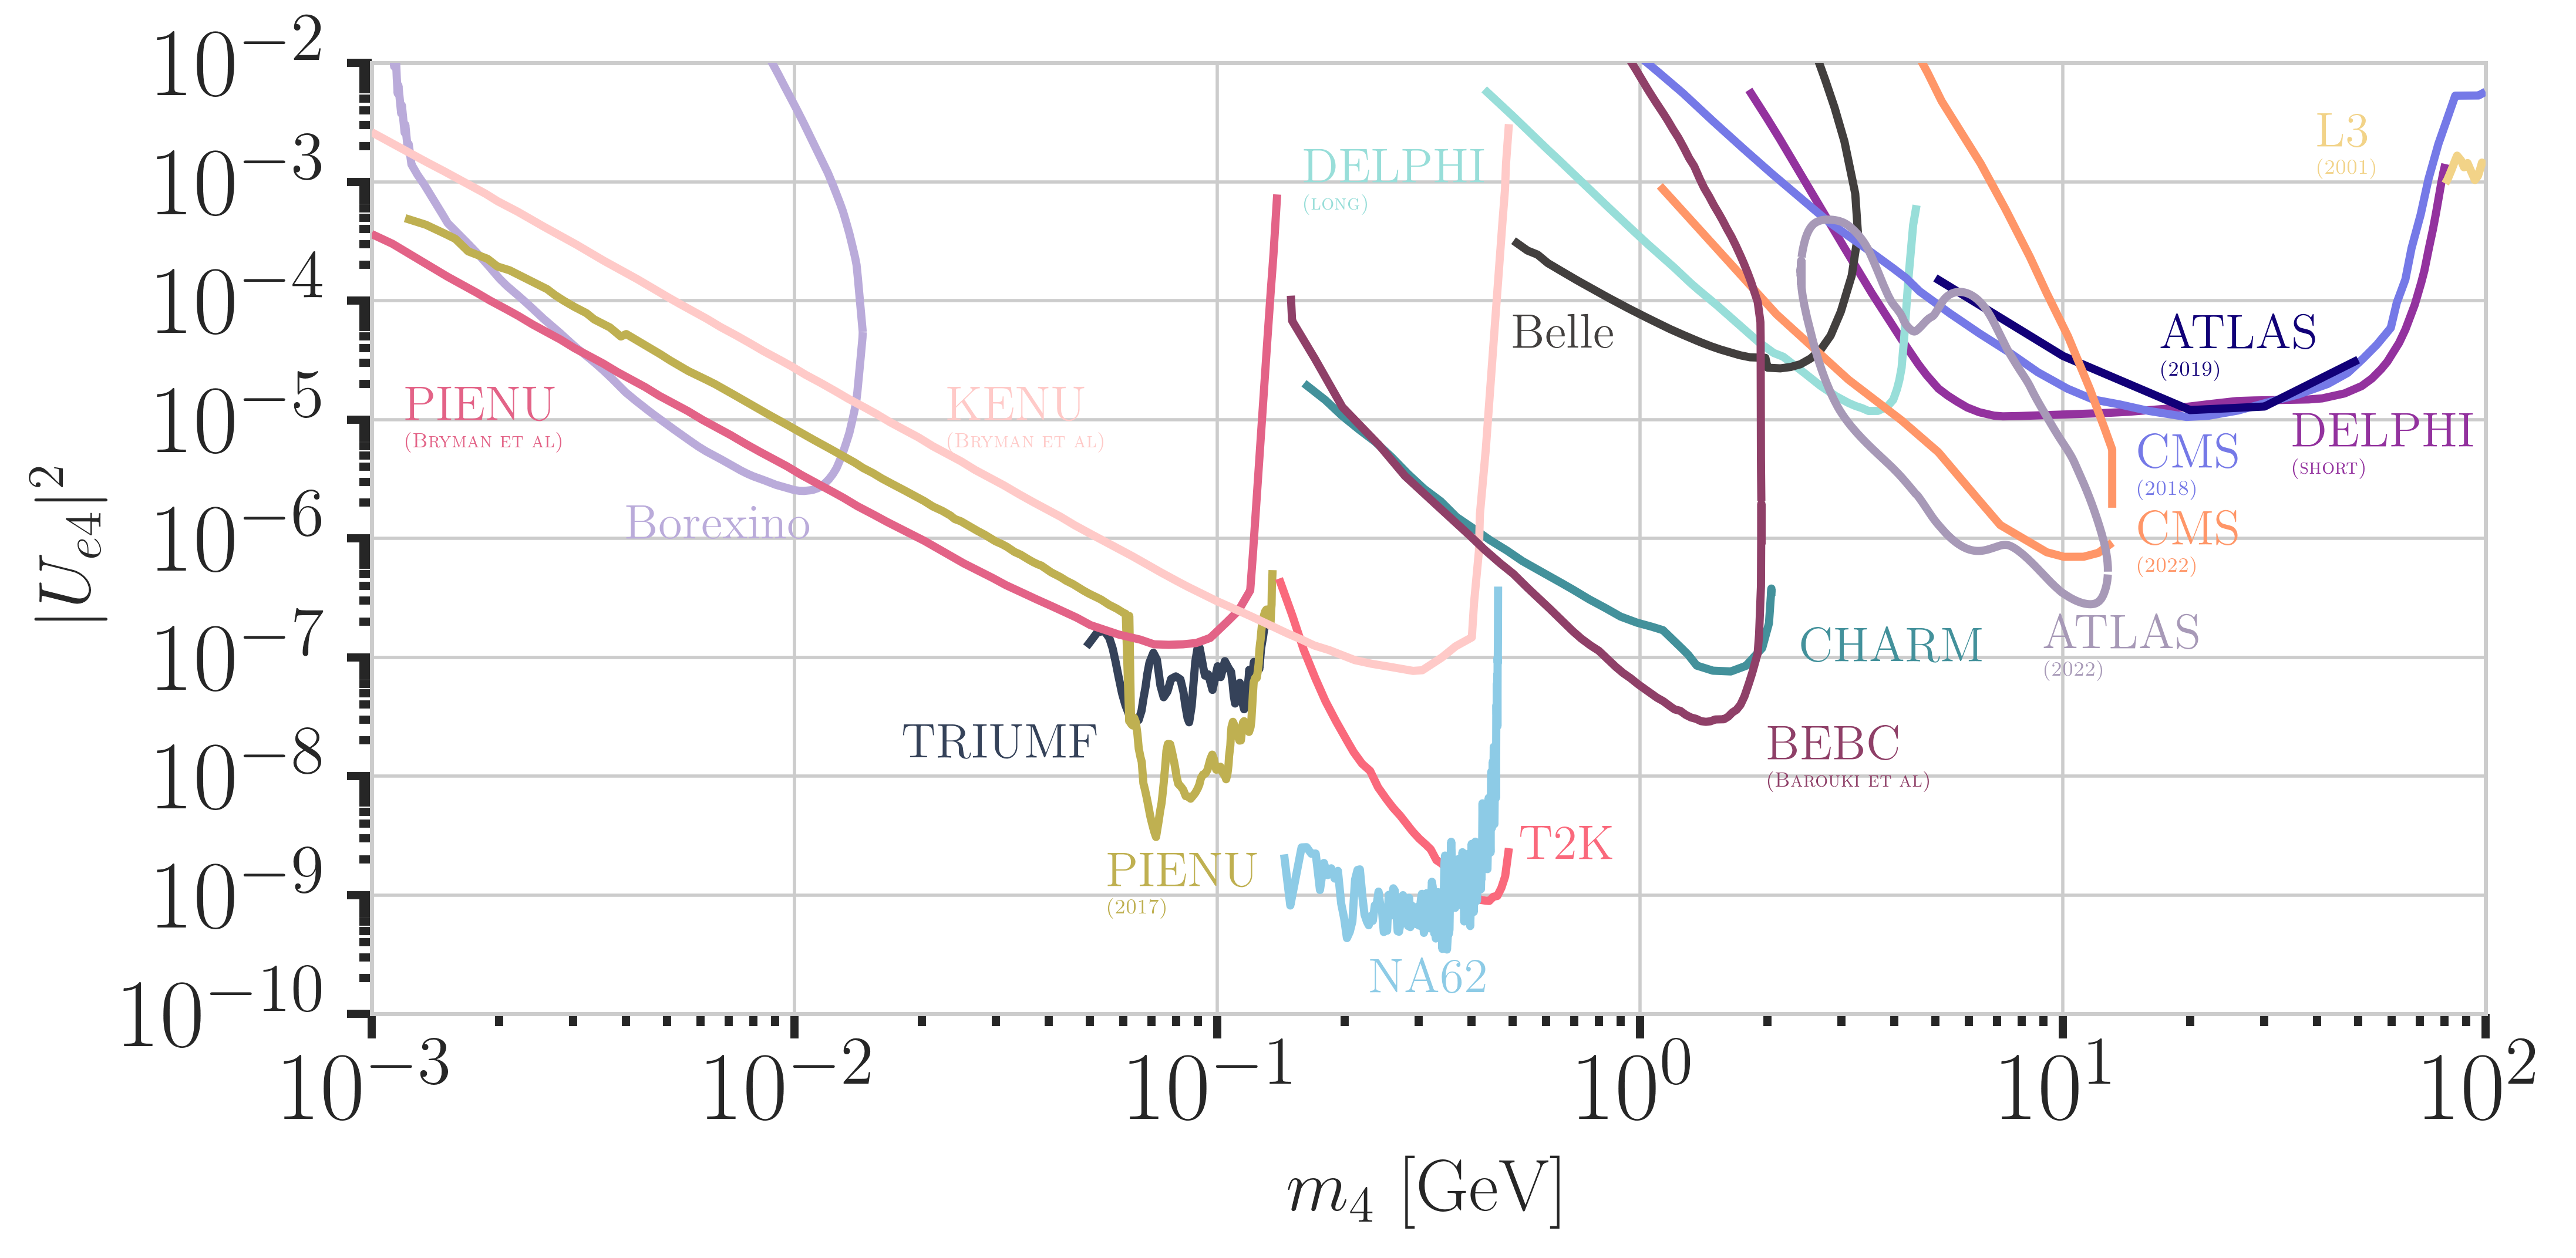
\includegraphics{figures/hnl_simulation/theory/UeN_majorana.png}
      \caption[Current leading $|U_{e4}^2|-m_4$ upper limits]{Current leading $|U_{e4}^2|-m_4$ upper limits from PIENU \cite{pienu_Bryman:2019bjg, PIENU:2017wbj}, BOREXINO \cite{Borexino:2013bot}, KENU \cite{pienu_Bryman:2019bjg}, TRIUMF \cite{triumf_ue4_Britton1992ImprovedSF}, NA62 \cite{NA62:2022pyf}, T2K \cite{T2K:2019jwa}, DELPHI \cite{DELPHI:1996qcc}, BEBC \cite{Barouki:2022bkt}, Belle \cite{Belle:2013ytx}, L3 \cite{L3:2001zfe}, CHARM \cite{CHARM:1983ayi}, ATLAS \cite{ATLAS:2019kpx, atlas_2022_HNL_PhysRevLett.131.061803}, CMS \cite{CMS:2018iaf, CMS:2022fut}, and NuTeV \cite{NuTeV:1999kej}. Modified from \cite{hoster_limitFernandez-Martinez:2023phj}.}
    \labfig{boundsUe}
\end{figure*}

Protons interacting with a target or a beam dump can produce pions, kaons, and heavy-quark hadrons, whose subsequent decays would also produce HNLs. Depending on the HNL lifetime in the specific model, the mass of the HNLs produced in beam dump experiments would be between \SI{1}{\mega\electronvolt} and \SI{4}{\gev} and they could decay at distances across several orders of magnitude, Experiments along the extracted beamline, which are using a spectrometer with particle identification, can search for unique decay signatures at displaced vertices. Example signatures\sidenote{The explicit channels and their decay width calculations used in this thesis are explained in detail in \refsec{custom_leptoninjector}.} are $\nu_4 \rightarrow l_\alpha \pi^+$, $\nu_4 \rightarrow \nu_\alpha l^+_\beta l^-_\beta$, or $\nu_4 \rightarrow \nu_\alpha \pi^0$ (or other neutral mesons) that cannot be explained by SM neutrinos. Here, $\nu_\alpha$ and $l_\alpha$ are the SM neutrino and charged lepton of flavor $\alpha \in \{e,\mu,\tau\}$, defined by which flavor the HNL couples to. $l^-_\beta$/$l^+_\beta$ is a charged lepton/antilepton pair of any flavor $\beta \in \{e,\mu,\tau\}$. Depending on the decay channel, a specific mixing can be probed. The other way of searching for HNLs with these interactions is to look for peaks in the missing mass spectrum, measured around the production vertex at the target, which usually is not possible for beam dumps, as the beam dump region is not calorimetrically instrumented. The HNL searches were pioneered by experiments at extracted beamlines, with \textit{PS191} \sidecite{Bernardi:1985ny} and \textit{CHARM} \sidecite{CHARM:1983ayi} establishing upper limits on \ue4, \um4, and combinations of them, at masses from \SIrange{10}{500}{\mega\electronvolt} at orders of $10^{-3}$ to $10^{-6}$. Since then, there has been and still is a large activity of searches for HNLs at extracted beamlines and at the lower mass end, the strongest bounds on \ue4 are set by \textit{PIENU} \sidecite{pienu_Bryman:2019bjg} at $\sim(10^{-4})$ around \SI{2}{\mega\electronvolt}, and at the higher mass end, the strongest bounds are set by \textit{NA62} \sidecite{NA62:2022pyf}, reaching down to $\sim10^{-9}$ at \SI{0.3}{\gev}. For \um4, the strongest bounds up to \SI{10}{\gev} are set by \textit{PSI} \sidecite{PSI_Daum:1987bg} at $\sim10^{-5}$, and reach down to $\sim(10^{-9})$ at \SI{0.3}{\gev}, by \textit{BNL-E949} \sidecite{BNL_E949:2014gsn}. The current strongest bounds are shown in \reffig{boundsUe} and \reffig{boundsUm}, where bounds from other type of experiments are also presented. Those will be discussed in the following.

Especially noteworthy are the results of analyses probing the mixing with the third lepton generation, \ut4, from \textit{NOMAD} \sidecite{NOMAD:2001eyx} and reinterpretations of the CHARM results and the BEBC results in the context of the mixing \ut4, where the latter places the most stringent limits from $10^{-3}$ to $10^{-6}$ in the \SIrange{0.1}{2}{\gev} range \sidecite{Orloff:2002de, Boiarska:2021yho, Barouki:2022bkt}. In \reffig{boundsUt} the current strongest bounds on \ut4 are shown.


\subsubsection{Collider Searches}

\begin{figure*}[t]
    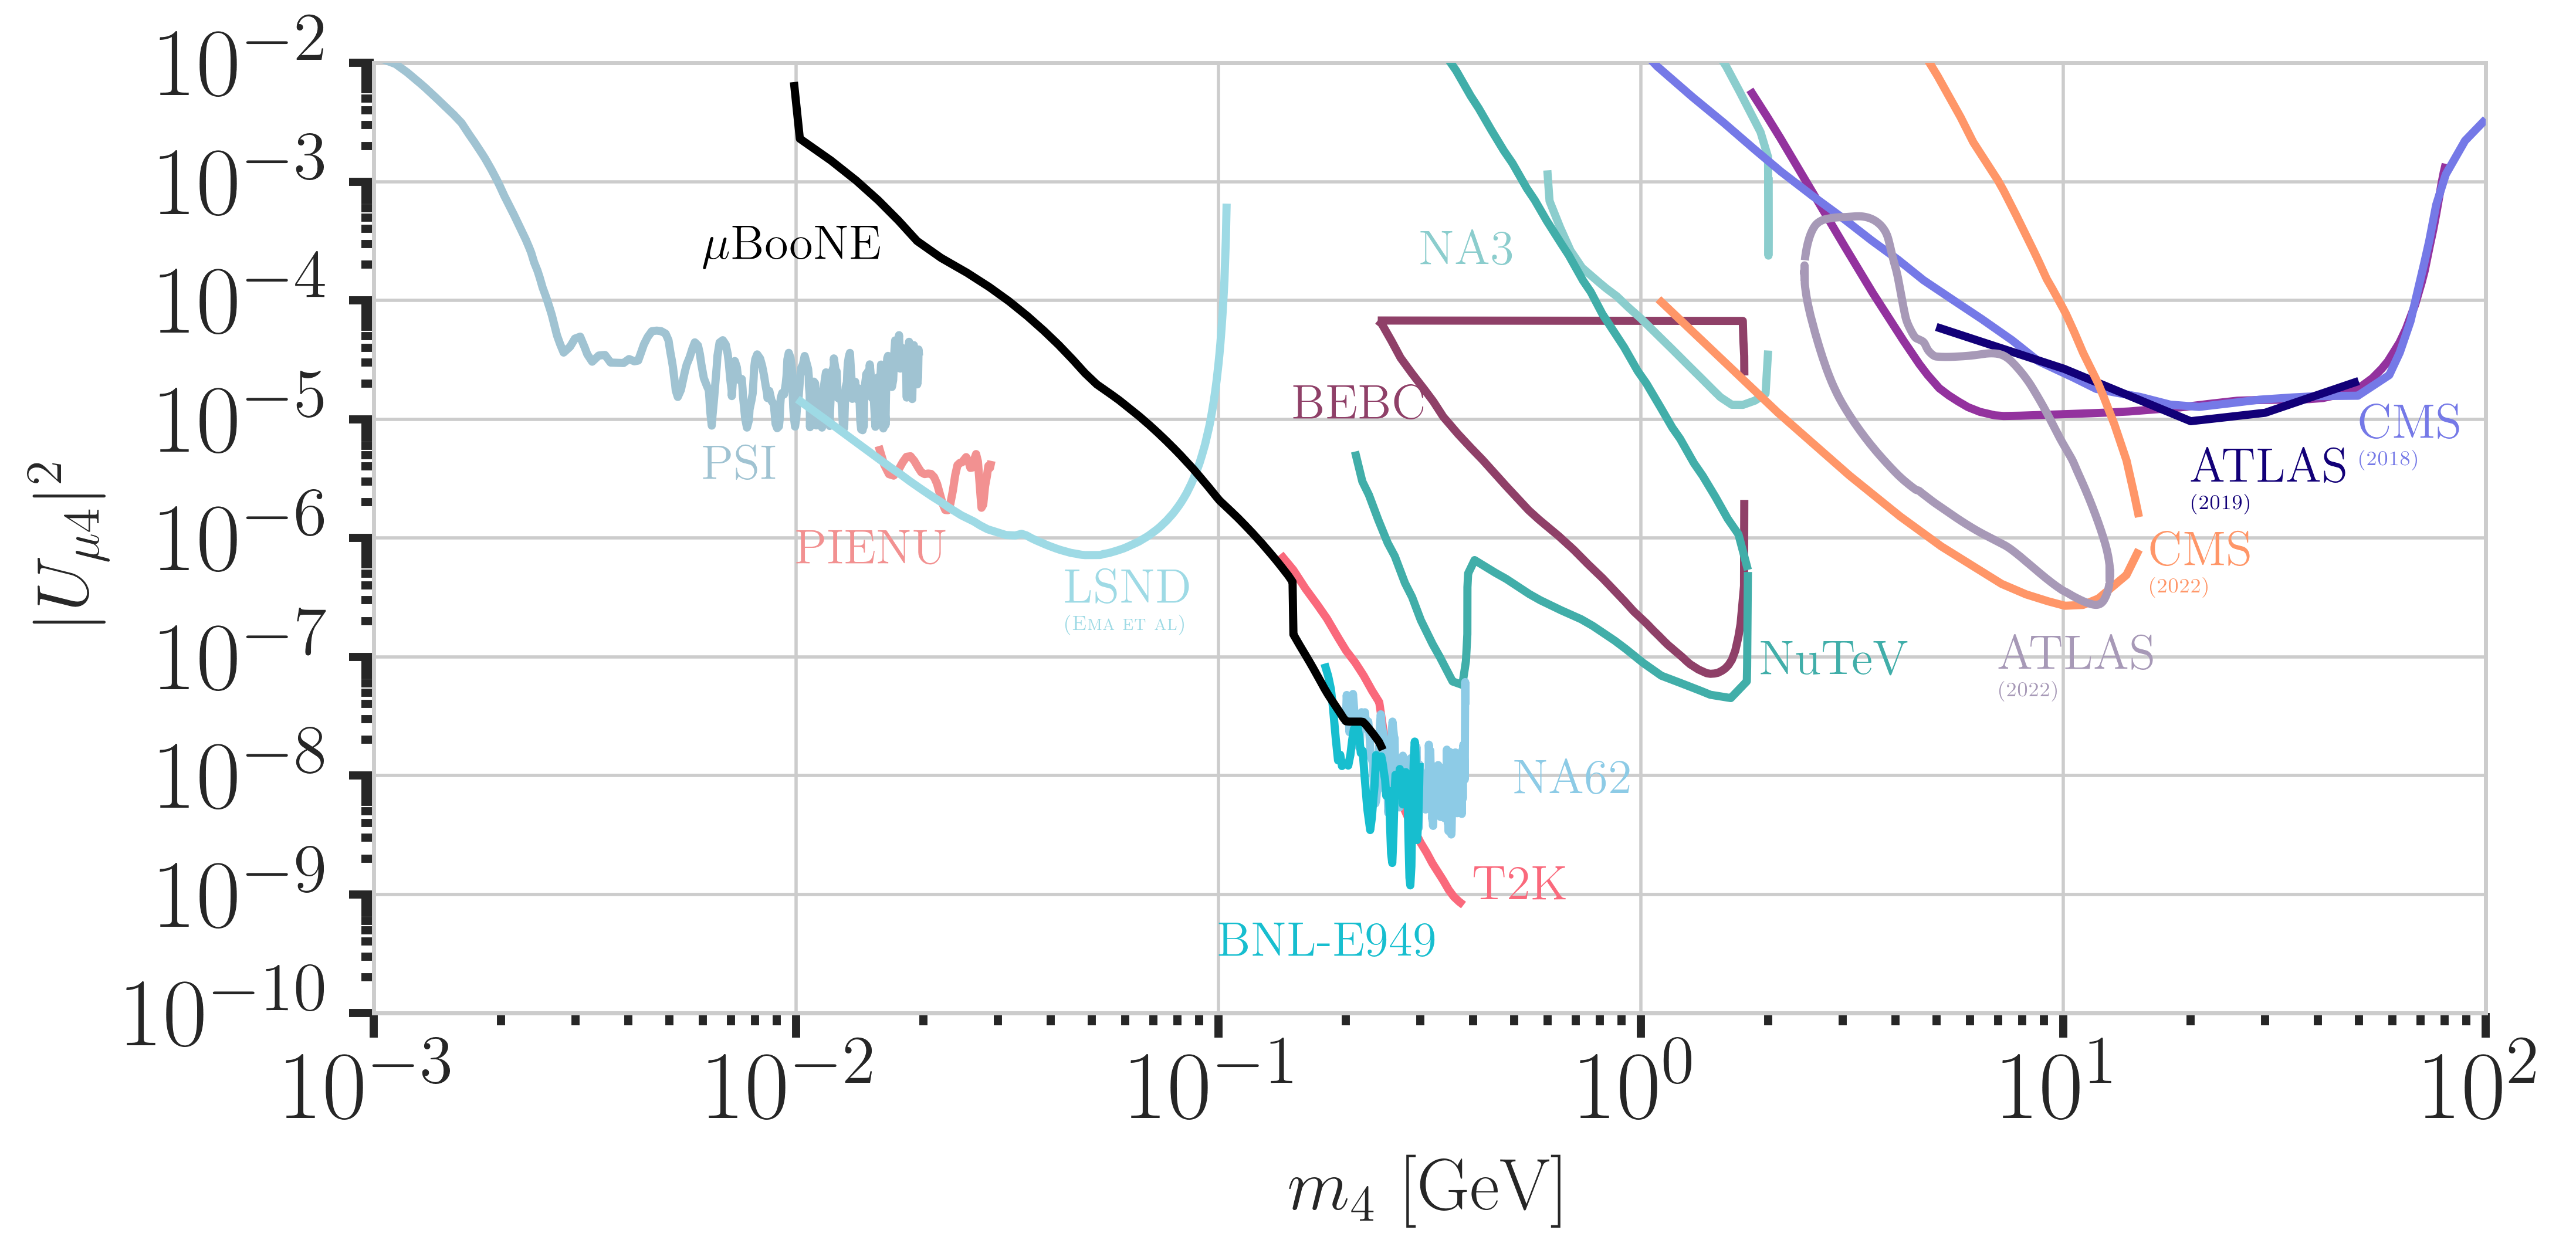
\includegraphics{figures/hnl_simulation/theory/UmuN_majorana.png}
      \caption[Current leading $|U_{\mu4}^2|-m_4$ upper limits]{Current leading $|U_{\mu4}^2|-m_4$ upper limits from PSI \cite{PSI_Daum:1987bg}, $\mu$BooNE \cite{MicroBooNE:2023eef}, PIENU \cite{pienu_Bryman:2019bjg}, LSND \cite{lsnd_Ema:2023buz}, BNL-E949 \cite{BNL_E949:2014gsn}, NA62 \cite{NA62:2022pyf}, T2K \cite{T2K:2019jwa}, BEBC \cite{BEBC_OG_COOPERSARKAR1985207},
      ATLAS \cite{ATLAS:2019kpx, atlas_2022_HNL_PhysRevLett.131.061803}, CMS \cite{CMS:2018iaf, CMS:2022fut}, NuTeV \cite{NuTeV:1999kej}, and NA3 \cite{NA3:1986ahv}. Modified from \cite{hoster_limitFernandez-Martinez:2023phj}.}
    \labfig{boundsUm}
\end{figure*}


So far, collider searches have been conducted at the \textit{large electron positron collider (LEP)} and at the \textit{large hadron collider (LHC)} in proton-proton mode. Strongest results are from the \textit{ATLAS} and \textit{CMS} experiments, which are nearly hermetic, general purpose detectors around the interaction point, and from the \textit{DELPHI} and the \textit{LHCb} experiments, which are forward detectors that can be used to search for new particles in decays of heavy particles produced. In the minimal model, HNLs in the \si{\gev} mass range can be produced through mass mixing in decays of heavy mesons, tau leptons, Z/W bosons, H bosons, or top quarks originating from the collisions. Depending on the dirac or majorana nature of the HNL, they can decay to lepton number conserving or lepton number violating channels.

Using prompt and displaced decays of the HNL, both ATLAS and CMS have set constraints on \ue4 and \um4 at the level of $10^{-4}$ to $10^{-6}$ in the mass range between \SIrange{1}{100}{\gev} \sidecite{ATLAS:2019kpx, atlas_2022_HNL_PhysRevLett.131.061803, CMS:2018iaf, CMS:2022fut}. The LHCb experiment has HNL search results at HNL masses below and above the W boson mass, where the low mass searches are using the decay channel $B^- \rightarrow \pi^+ \mu^- \mu^-$, setting limits at the $10^{-3}$ level for \um4 in the mass range of \SIrange{0.5}{3.5}{\gev} \sidecite{Shuve:2016muy}. At high masses, the $W^+ \rightarrow \mu^- \mu^\pm$jet channel is used to set limits at the order of $10^{-3}$ to $10^{-2}$ for \um4 in the mass range of \SIrange{5}{50}{\gev} in the LNC channel and at the order of $10^{-4}$ to $10^{-3}$ in the LNV channel \sidecite{LHCb:2020wxx}. Using hadronic $Z^0$ decays, searches for short- and long-lived HNLs have been conducted with the \textit{DELPHI} detector setting upper limits of the order of $10^{-5}$ for mixing to any SM flavor in the mass range from \SIrange{3.5}{50}{\gev} \sidecite{DELPHI:1996qcc}. 


\subsubsection{Nuclear Decays Measurements}

\begin{figure*}[t]
    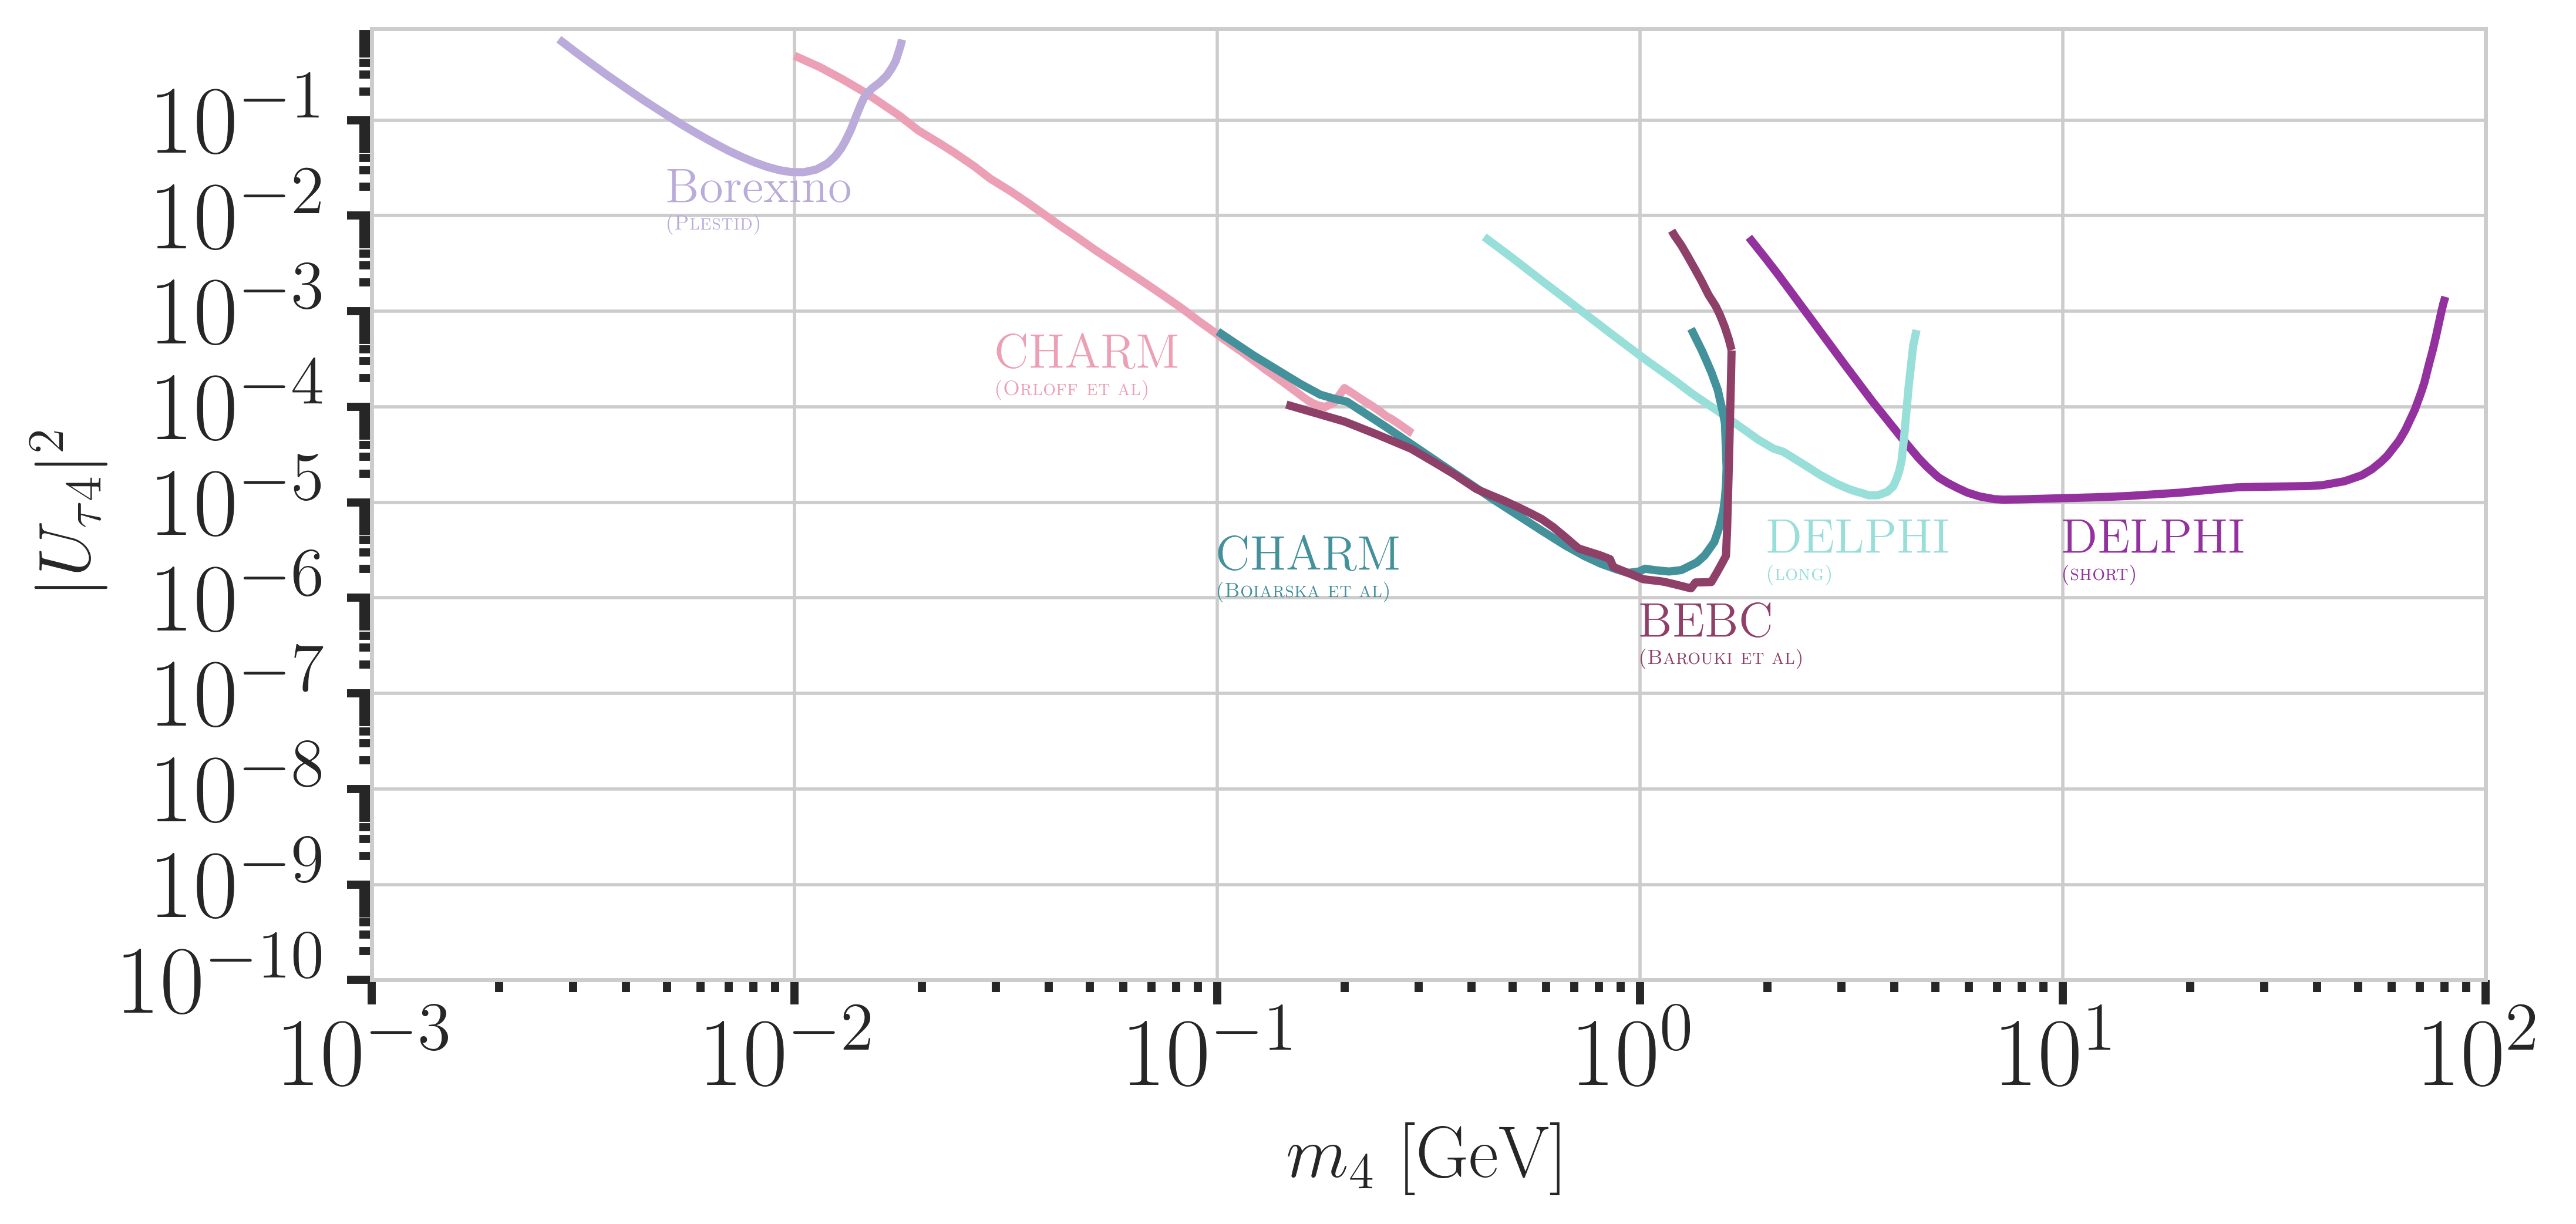
\includegraphics{figures/hnl_simulation/theory/UtauN_majorana.png}
      \caption[Current leading $|U_{\tau4}^2|-m_4$ upper limits]{Current leading $|U_{\tau4}^2|-m_4$ upper limits from BOREXINO \cite{Plestid:2020vqf}, CHARM \cite{Orloff:2002de, Boiarska:2021yho}, DELPHI \cite{DELPHI:1996qcc}, and BEBC \cite{Barouki:2022bkt}. Modified from \cite{hoster_limitFernandez-Martinez:2023phj}.}
    \labfig{boundsUt}
\end{figure*}

A novel approach of searching for irregularities in energy-momentum conservation measurements in nuclear reactions might be a viable way of searching for HNLs, as they could be interpreted as constraints on \ue4 and $m_4$.

Kinks in \textbf{beta decay} spectra would show up at $Q-m_4c^2$, where the HNL mass, $m_4$, can be measured between the lower energy detection threshold and the energy released in the decay, which is called $Q$ value. Analyses using the tritium decay, with $Q=\SI{18.6}{\kilo\electronvolt}$, are planned in \textit{KATRIN} \sidecite{KATRIN:2001ttj} and \textit{TRISTAN} \sidecite{Mertens_2019} in the \SIrange{1}{18}{\kilo\electronvolt} range. Their projected statistical limits are around $10^{-7}$ for \ue4, but will require further detector upgrades \cite{Mertens_2019}. A first result from KATRIN measurements during commissioning sets limits at the order of $10^{-2}$ to $10^{-3}$ in the mass range of \SIrange{0.1}{1.6}{\kilo\electronvolt} \sidecite{KATRIN:2022spi}. \textit{DUNE} is planning to measure the ionization charge of atmospheric argon decays, with $Q=\SI{565}{\kilo\electronvolt}$, to probe \ue4 at in the \SIrange{20}{450}{\kilo\electronvolt} mass range. The projected sensitivity is at the $10^{-5}$ level, and might improve to $10^{-7}$ with additional detector improvements \sidecite{DUNE:2020ypp}.

To test for the existence of HNLs using \textbf{electron capture} measurements, total energy-momentum reconstruction of all non-neutrino final states is needed. Electron capture is a pure two-body decay process, where the recoiling atom and the electron neutrino are the only final state particles, but additional energy is carried away by the de-excitation x-ray or auger electron. The energy-momentum conservation can be probed by measuring the atom and the associated de-excitation products. The mixing \ue4 can be probed by looking for a separated non-zero missing mass peak. The \textit{BeEST} experiment has set limits at the $10^{-4}$ level in the \SIrange{100}{850}{\kilo\electronvolt} mass range, using berillium-7, which has a $Q$ value of \SI{862}{\kilo\electronvolt}. After planned upgrades to the experiment, the sensitivity is expected to improve to the $10^{-7}$ level \sidecite{BeEST_Friedrich:2020nze}.

\textbf{Reactor searches} up to \SI{12}{\mega\electronvolt} in mass are possible at short baseline experiments using commercial or research reactors, which are a strong source of electron antineutrinos and could therefore also produce HNLs if \ue4 is non-zero. Visible decay channels at these energies are $\nu_4 \rightarrow \nu_e e^+ e^-$, $\nu_4 \rightarrow \nu \gamma$, and $\nu_4 \rightarrow \nu \gamma \gamma$, where the first dominates. The first analysis in this field, reports limits at the $10^{-4}$ level in the \SIrange{2}{7}{\mega\electronvolt} mass range \sidecite{de59e8a4525048378bfd5f3973e2d6ad}.


\subsubsection{Atmospheric and Solar Neutrinos}

Natural sources of neutrinos are provided up to \SI{20}{\mega\electronvolt} by the sun and up to 100s of \si{\gev} by neutrino production in the atmosphere. Both fluxes contain all flavors of neutrinos, due to mixing and oscillations, and can therefore be used to directly probe the mixings with $\nu_e$, $\nu_\mu$, and $\nu_\tau$. Depending on the HNL mass and the strength of the mixing, which both govern the decay length, different signatures can be used to experimentally access large regions of the HNL parameter space. The strength of the mixing determines the total rate of HNL events, which is additionally affected by whether solely the minimal mass mixing is assumed, or also more complicated mixing scenarios, like the dipole portal, are considered.

So far, only very few analyses exist, which are performed by the experimental collaborations themselves. Several external theoretical groups have predicted the expected sensitivities to HNLs, produced from solar or atmospheric neutrinos, based on various coupling scenarios and decay lengths. A selection of the potential analyses will be discussed in the following.

For very long-lived particles, \textbf{production inside the sun} can be used as a source to search for HNLs in detectors on earth. This will only allow production through non-zero \ue4, because the initial solar neutrino flux is only $\nu_e$. By searching for HNL decays to a SM neutrino and an electron positron pair $\nu_4 \rightarrow \nu_e e^+ e^-$ and comparing to the expected inter planetery positron flux, \textit{Borexino} has placed the strongest limits on the mixing \ue4 at the order of $10^{-5}$ in the few \si{\mega\electronvolt} mass range \sidecite{Borexino:2013bot}.

For HNL decay length scales of the order of the Earth's diameter, HNL \textbf{up-scattering outside the detector} is possible, where a neutrino from the solar or the atmospheric neutrino flux scatters in the Earth and transfers some kinetic energy to the HNL, which can then later decay inside the detector. For HNL masses below \SI{18}{\mega\electronvolt} produced from solar neutrinos, limits were derived using the Borexino data for purely tau coupling through mass mixing \sidecite{Plestid:2020vqf} and for all flavor coupling through the dipole portal \sidecite{Plestid:2020ssy}. At similar decay length scales, the HNL could also be produced directly in the atmosphere, but neither this channel, nor the production anywhere in the Earth from atmospheric neutrinos has been investigated yet.

If the HNL decay lengths are sufficiently short, \textbf{production and decay in the detector} can happen and the observation of two vertices could be used to constrain the mixing parameters. In principle, this could be possible with any neutrino flavor produced in the sun or the atmosphere, but so far only theoretical studies have been performed for mass-mixing and dipole-portal couplings for the atmospheric neutrino detectors IceCube \sidecite{Coloma:2017ppo,Coloma:2019qqj} and \textit{Super-K}, \textit{Hyper-K}, and Dune \sidecite{Atkinson:2021rnp, Coloma:2020lgy}. Due to the high complexity of these experiments, several simplified assumptions were made in the studies, which might not hold in reality, and the results should be taken with caution. For reliable sensitivity estimates and limits the collaborations should perform their own analyses.


\section{Atmospheric Neutrinos as Source of Heavy Neutral Leptons} \labsec{hnl_theory}

This work focuses on the search for HNLs using atmospheric neutrinos as source for the production and decay inside the IceCube detector. The following sections will give a brief overview of the production of neutrinos in the atmosphere and the oscillations they undergo, before discussing the expected signatures of HNLs in the detector, where they are produced from the incoming neutrinos and subsequently decay.


\subsection{Production of Neutrinos in the Atmosphere}

The analysis performed in this work is based on the sample of neutrinos observed in IceCube DeepCore at energies below \SI{100}{\gev}. At these energies, the flux exclusively originates in the Earth's atmosphere. Highly relativistic cosmic rays (protons and heavier nuclei \sidecite{PhysRevD.98.030001}) interact in the upper atmosphere, producing showers of secondary particles. Neutrinos are produced in decays of charged pions and kaons ($\pi$ and $K$ mesons) present in those showers, where the dominant contribution comes from the decay chain
\begin{equation}
    \begin{split}   
        \pi^\pm &\rightarrow \mu^\pm + \nu_\mu(\bar{\nu}_\mu)\;, \\
        \mu^\pm &\rightarrow e^\pm + \bar{\nu}_\mu(\nu_\mu) + \nu_e(\bar{\nu}_e)
        \;,
    \end{split}
    \labeq{pion_decay}
\end{equation}
where muon neutrinos $\nu_\mu$ and muons $\mu^\pm$ are produced in the first decay and both electron and muon neutrinos $\nu_{e/\mu}$ are produced in the second decay. Atmospheric muons, which are also produced in these decays, are the main background component for IceCube DeepCore analyses.

\begin{figure}
    \centering
    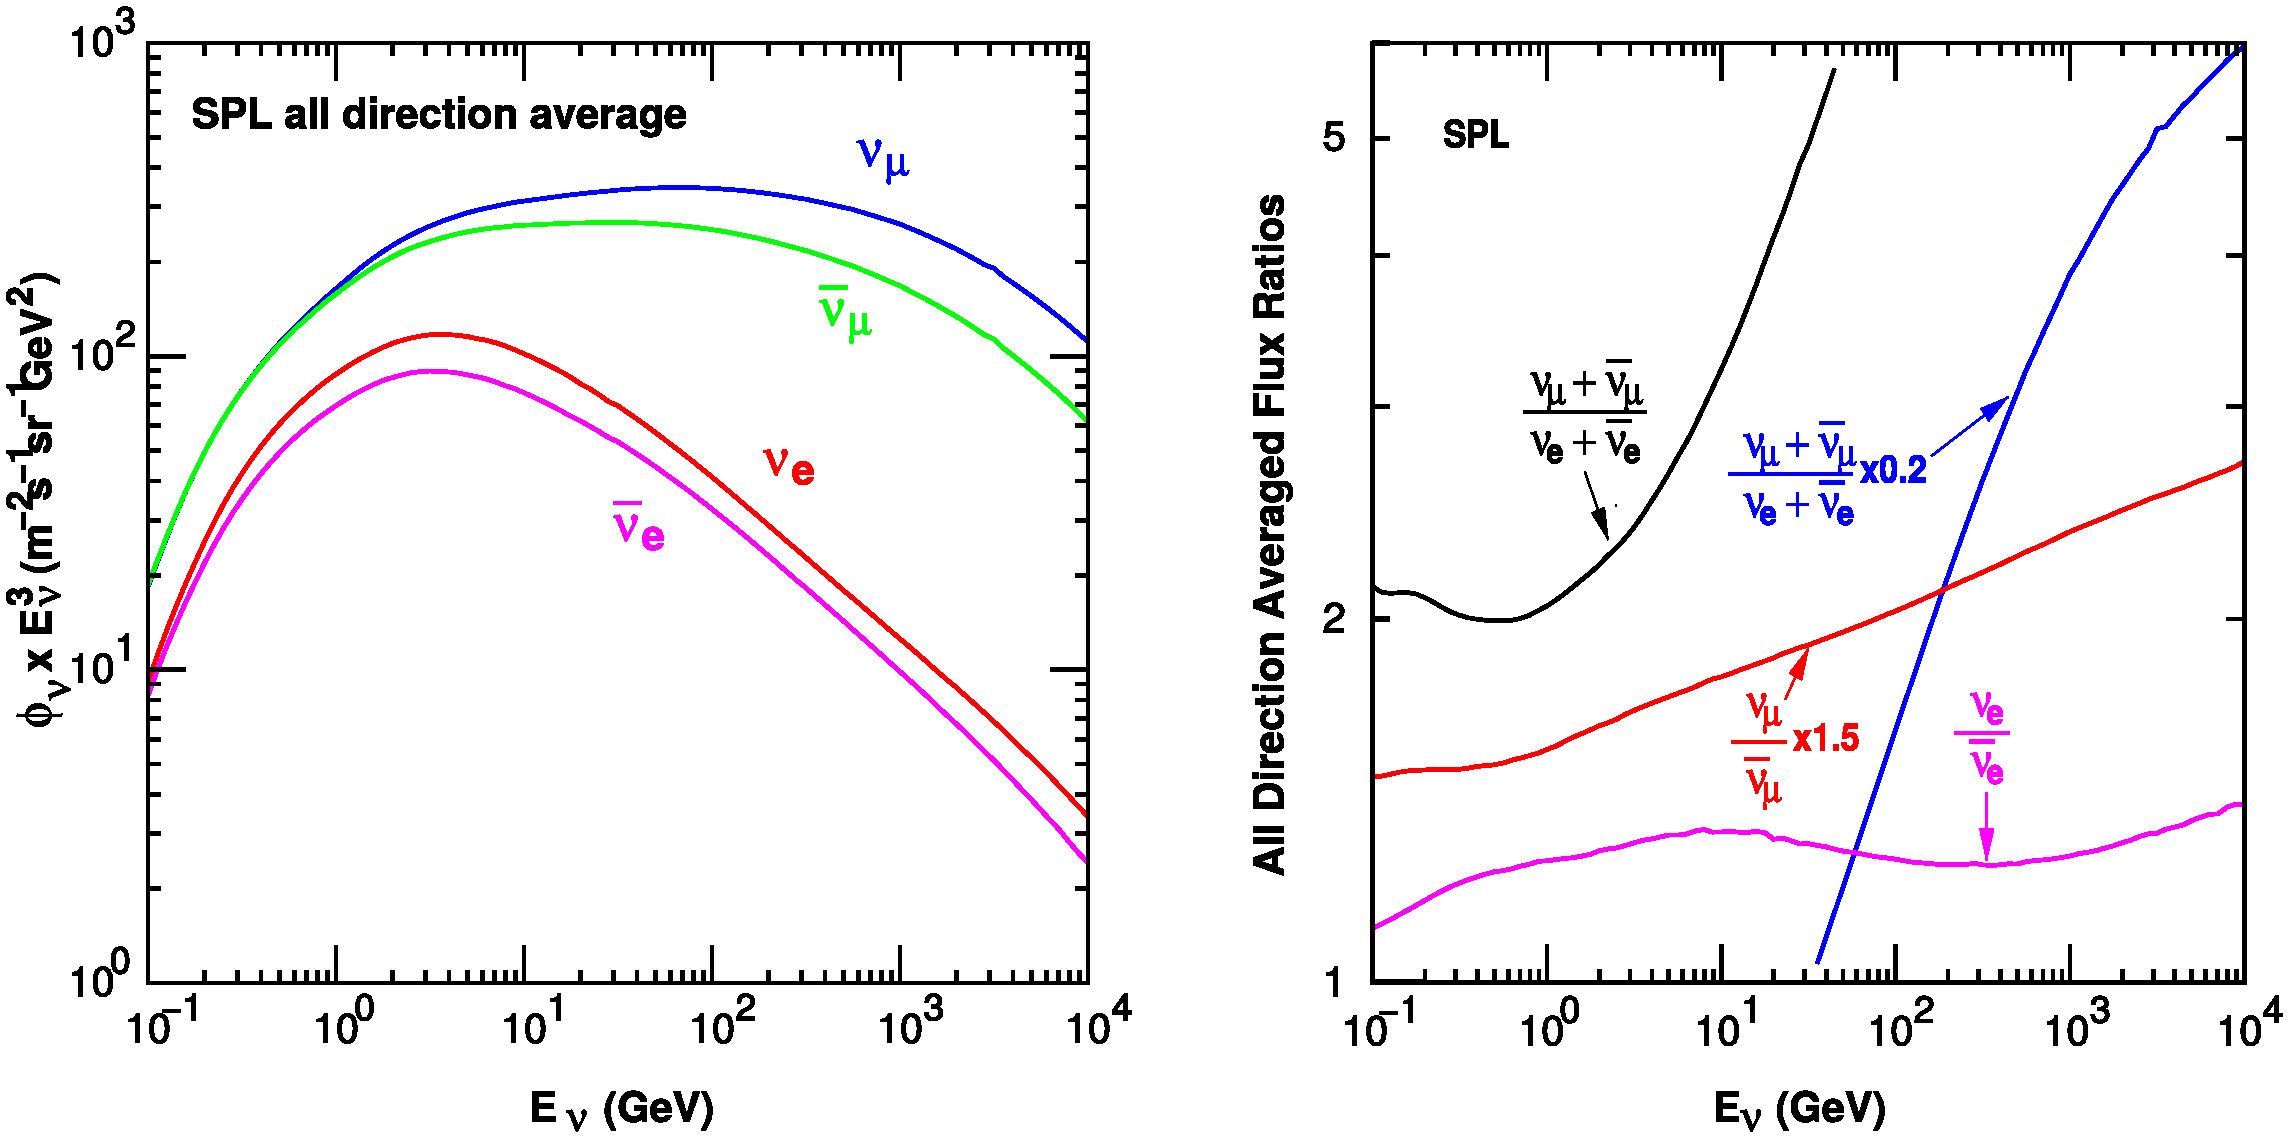
\includegraphics[width=1.0\textwidth]{figures/neutrinos_properties/Honda_alldir-spl_copy.pdf}
    \caption[Atmospheric neutrino fluxes]{The atmospheric fluxes of different neutrino flavors as a function of energy (left) and the ratios between muon neutrinos and electron neutrinos as well as the ratios between neutrinos and antineutrinos for both those flavors (right). Results from the calculations performed for the geographic South Pole, taken from \cite{PhysRevD.92.023004_Honda_Flux}.}
    \labfig{honda_flux}
\end{figure}

The different atmospheric flux components are shown in \reffig{honda_flux} (left), for a much broader energy range than relevant for this work. Both neutrinos and antineutrino fluxes are shown for electron  and muon neutrinos and all fluxes are the directionally averaged expectation calculated at the South Pole. Muon neutrinos are dominating the flux and from \refeq{pion_decay} the naive assumption would be that the ratio between muon and electron neutrinos is $(\nu_\mu+\bar{\nu}_\mu)/(\nu_e+\bar{\nu}_e)=2$. This is roughly true at energies below \SI{1}{\gev}, where all muons decay in flight, but at larger energies muons can reach the detector before decaying, which increases the ratio to approximately 10:1 at around \SI{100}{\gev}. Additionally, kaon decays start to contribute which also increases the number of muons and muon neutrinos. The increasing ratio can be seen in \reffig{honda_flux} (right), which also shows the ratio between neutrinos and antineutrinos for both flavors.

Charged mesons heavier than the tau can also be produced in cosmic ray interactions. Their decays to tau neutrinos or direct production of taus in cosmic ray interactions lead to the production of tau neutrinos. At the energies relevant for this work however, the resulting tau neutrino flux is negligible as compared to the muon neutrino flux \sidecite{2015EPJWC..9908001F_lepton_fluxes} and is not considered in the analysis. This is because both charged mesons and tau particles are much heavier than pions and kaons and therefore their production is suppressed at high energies.


\subsection{Neutrino Oscillations} \labsec{neutrino_oscillations}

Describing neutrinos in their mass state as introduced in \refsec{neutrino_mass_mixing} is crucial to understanding their propagation through space and time and to explaining neutrino oscillations. Oscillations mean that a neutrino changes from its initial flavor, that it was produced with, to another flavor and back after traveling a certain distance.

The neutrino propagation in vacuum can be expressed by applying a plane wave approach, where the mass eigenstates evolve as
\begin{equation}
    \ket{\nu_k(t)} = e^{-iE_kt/\hbar}\ket{\nu_k}
    \;.
    \labeq{flavor_time_evol}
\end{equation}
The energy of the mass eigenstate $\ket{\nu_k}$ is $E_k=\sqrt{\vec{p}^2c^2+m_k^2c^4}$, with momentum $\vec{p}$ and mass $m_k$, $\hbar$ is the reduced Planck constant, and c is the speed of light in vacuum. A neutrino is produced as a flavor eigenstate $\ket{\nu_\alpha}$ in a CC weak interaction, but its propagation happens as the individual mass states it is composed of. The probability of finding the neutrino with initial flavor $\ket{\nu_\alpha}$ in the flavor state $\ket{\nu_\beta}$ after the time $t$ is calculated as
\begin{equation}
    P_{\nu_\alpha \rightarrow \nu_\beta}(t)
    =
    \big|\braket{\nu_\beta|\nu_\alpha(t)}\big|^2
    \;,
    \labeq{fermis_golden_rule}
\end{equation}
by applying Fermi's Golden Rule \sidecite{1927RSPSA.114..243D}, which defines the transition rate from one eigenstate to another by the strength of the coupling between them. This coupling strength is the square of the matrix element and using the fact that the mixing matrix is unitary ($U^{-1}=U^\dagger$) to describe the mass eigenstates as flavor eigenstates, we find the time evolution of the flavor state $\ket{\nu_\alpha(t)}$, which can be inserted into \refeq{fermis_golden_rule} to find the probability as
\begin{equation}
    P_{\nu_\alpha \rightarrow \nu_\beta}(t)
    =
    \sum_{j,k}U^*_{\beta j}U_{\alpha j}U_{\beta k}U^*_{\alpha k}e^{-i(E_k-E_j)t/\hbar}
    \;.
    \labeq{probability_raw}
\end{equation}
The indices $j$ and $k$ run over the mass eigenstates.

We can approximate the energy as
\begin{equation}
    E_k \approx E+\frac{c^4m^2_k}{2E} \hspace{0.25cm} \longrightarrow \hspace{0.25cm} E_k-E_j \approx \frac{c^4\Delta m^2_{kj}}{2E}
    \;,
\end{equation}
for very small masses compared to the kinetic energy $E\gg m_kc^2$. Here, $\Delta m^2_{kj}=m^2_k-m^2_j$ is the mass-squared splitting between states $k$ and $j$, and $E$ is the energy of the wavepacket to be detected (flavor eigenstate). Replacing the time in \refeq{probability_raw} by the distance traveled by relativistic neutrinos $t\approx L/c$ we get
\begin{equation}
    \begin{split}
        P_{\nu_\alpha \rightarrow \nu_\beta}(t)
        = 
        \delta_{\alpha \beta}
        -
        4\sum_{j>k}&\textbf{Re}(U^*_{\beta j}U_{\alpha j}U_{\beta k}U^*_{\alpha k})\textrm{sin}^2\Big( \frac{c^3\Delta m^2_{kj}}{4E\hbar}L \Big) \\
        +
        2\sum_{j>k}&\textbf{Im}(U^*_{\beta j}U_{\alpha j}U_{\beta k}U^*_{\alpha k})\textrm{sin}^2\Big( \frac{c^3\Delta m^2_{kj}}{4E\hbar}L \Big)
        \;,
    \end{split}
    \labeq{probability_detailed}
\end{equation}
which is called the survival probability if $\alpha=\beta$, and the transition probability if $\alpha\neq\beta$. Once again, this probability is only non-zero if there are neutrino mass eigenstates with masses greater than zero. Additionally, there must be a mass-squared difference $\Delta m^2$ and non-zero mixing between the states. Since we assumed propagation in vacuum in \refeq{flavor_time_evol}, the transition and survival probabilities correspond to vacuum mixing.

{\renewcommand{\arraystretch}{0.7}
\begin{margintable}[3cm]
    \footnotesize
    \begin{tabular}{ cc }
    \hline\hline    
    Parameter & Global Fit \\
    \hline\hline    
    $\theta_{12}$ [\si{\degree}] & $33.41^{+0.75}_{-0.72}$ \\
    $\theta_{13}$ [\si{\degree}] & $8.54^{+0.11}_{-0.12}$ \\
    $\theta_{23}$ [\si{\degree}] & $49.1^{+1.0}_{-1.3}$ \\
    \hline
    $\Delta m^2_{21}$ [$10^{-5}$\si{\electronvolt^2}] & $7.41^{+0.21}_{-0.20}$ \\
    $\Delta m^2_{31}$ [$10^{-3}$\si{\electronvolt^2}] & $2.511^{+0.028}_{-0.027}$ \\
    \hline
    $\delta_{CP}$ [\si{\degree}] & $197^{+42}_{-25}$ \\
    \hline
    \end{tabular}
\caption[Global fit neutrino mixing parameter results]{Results from the latest global fit of neutrino mixing parameters from \cite{nufit_5.2}.}
\labtab{nufit_5.2}
\end{margintable}
}

The mixing matrix can be parameterized as \sidecite{PhysRevD.98.030001}
\begin{equation}
    U=\left( 
    \begin{matrix}
        1 & 0 & 0 \\
        0 & c_{23}  & s_{23} \\
        0 & -s_{23} & c_{23} 
    \end{matrix}
    \right) 
    \left( 
    \begin{matrix}
        c_{13} & 0 & s_{13}e^{-i\delta_{CP}} \\
        0 & 1 & 0\\
        -s_{13} e^{i\delta_{CP}} & 0 & c_{13}
    \end{matrix}
    \right) 
    \left( 
    \begin{matrix}
        c_{12} & s_{12} & 0 \\
        -s_{12} & c_{12} & 0\\
        0 & 0 & 1
    \end{matrix} 
    \right)  
    \;,
    \labeq{parameterized_PMNS_matrix}
\end{equation}
where $c_{ij}=\cos\theta_{ij}$ and $s_{ij}=\sin\theta_{ij}$ are cosine and sine of the mixing angle $\theta_{ij}$, that defines the strength of the mixing between the mass eigenstates $i$ and $j$, and $\delta_{CP}$ is the neutrino CP-violating phase. Experiments are sensitive to different mixing parameters, depending on the observed energy range, neutrino flavor, and the distance between the source and the detector $L$, commonly referred to as \textit{baseline}. To be able to resolve oscillations the argument
\begin{equation}
    \frac{\Delta m^2L}{4E}
    \labeq{oscillation_argument}
\end{equation}
should be at the order of 1. This divides experiments into ones that are sensitive to very slow oscillations from $\Delta m^2_{21}\approx\mathcal{O}(10^{-5}\si{\electronvolt^2})$ and ones that are sensitive to faster oscillations from $\Delta m^2_{31}\approx\mathcal{O}(10^{-3}\si{\electronvolt^2})$.
Relevant for this work are the parameters that can be measured at the earths surface using atmospheric neutrinos, which are $\Delta m^2_{31}$, $\theta_{23}$, and $\theta_{13}$, because the flux is primarily composed of muon neutrinos and antineutrinos. Applying the parameterization from \refeq{parameterized_PMNS_matrix} to \refeq{probability_detailed} and using the fact that $\theta_{13}$ is small and $\theta_{12}$ is close to $\pi/4$, the survival probability of muon neutrinos can be approximated as
\begin{equation}
    \begin{split}
        P_{\nu_\mu \rightarrow \nu_\mu}
        \simeq 
        1 - 4 |U_{\mu3}|^2(1-|U_{\mu3}|^2)\sin^2\Big( \frac{\Delta m^2_{31}L}{4E} \Big) \\
        \simeq
        1 - \sin^2\Big( 2\theta_{23} \Big)\sin^2\Big( \frac{\Delta m^2_{31}L}{4E} \Big)
        \;,
    \end{split}
    \labeq{probability_muon_survival}
\end{equation}
while the tau neutrino appearance probability is
\begin{equation}
    \begin{split}
        P_{\nu_\mu \rightarrow \nu_\tau}
        \simeq 
        4 |U_{\mu3}|^2|U_{\tau3}|^2\sin^2\Big( \frac{\Delta m^2_{31}L}{4E} \Big) \\
        \simeq
        \sin^2\Big( 2\theta_{23} \Big)\sin^2\Big( \frac{\Delta m^2_{31}L}{4E} \Big)
        \;.
    \end{split}
    \labeq{probability_tau_appearance}
\end{equation}
The latest global fit \sidecite{nufit_5.2} of all the parameters is shown in \reftab{nufit_5.2}.


\subsection{Neutrino Interactions with Nuclei} \labsec{neutrino_interactions}

The neutrino detection principle of IceCube DeepCore is explained in \refch{icecube} and relies on the weak interaction processes between neutrinos and the nuclei of the Antarctic glacial ice. At neutrino energies above \SI{5}{\gev}, the cross-sections are dominated by \textbf{\textit{deep inelastic scattering (DIS)}}, where the neutrino is energetic enough to resolve the underlying structure of the nucleons and interact with one of the composing quarks individually. As a result the nucleon breaks and a shower of hadronic secondary particles is produced. Depending on the type of interaction, the neutrino either remains in the final state for NC interactions or is converted into its charged lepton counterpart for CC interactions. The CC DIS interactions have the form
\begin{equation}
    \begin{split}
        \nu_\alpha + N \rightarrow l^-_\alpha + X \;, \\
        \bar{\nu}_\alpha + N \rightarrow l^+_\alpha + X \;, \\
        \;,
    \end{split}
    \labeq{dis_cc}
\end{equation}
where $\nu_\alpha$/$\bar{\nu}_\alpha$ and $l^-_\alpha$/$l^+_\alpha$ are the neutrino/antineutrino and its corresponding lepton/antilepton for $\alpha=e,\mu,\tau$.$N$ is the nucleon and $X$ stands for any set of final state hadrons. The NC DIS interactions are
\begin{equation}
    \begin{split}
    \nu_\alpha + N & \rightarrow \nu_\alpha + X \; \rm{and} \\
    \bar{\nu}_\alpha + N & \rightarrow \bar{\nu}_\alpha + X \;. \\
    \end{split}
    \labeq{dis_nc}
\end{equation}
DIS interactions have a roughly linear energy dependent cross-section above $\sim$\SI{20}{\gev} and are well measured and easy to theoretically calculate. They are the primary interaction channel for neutrinos detected with IceCube. \reffig{dis_feynman} shows the Feynman diagrams for both processes.

\begin{figure}[h]
    \centering
    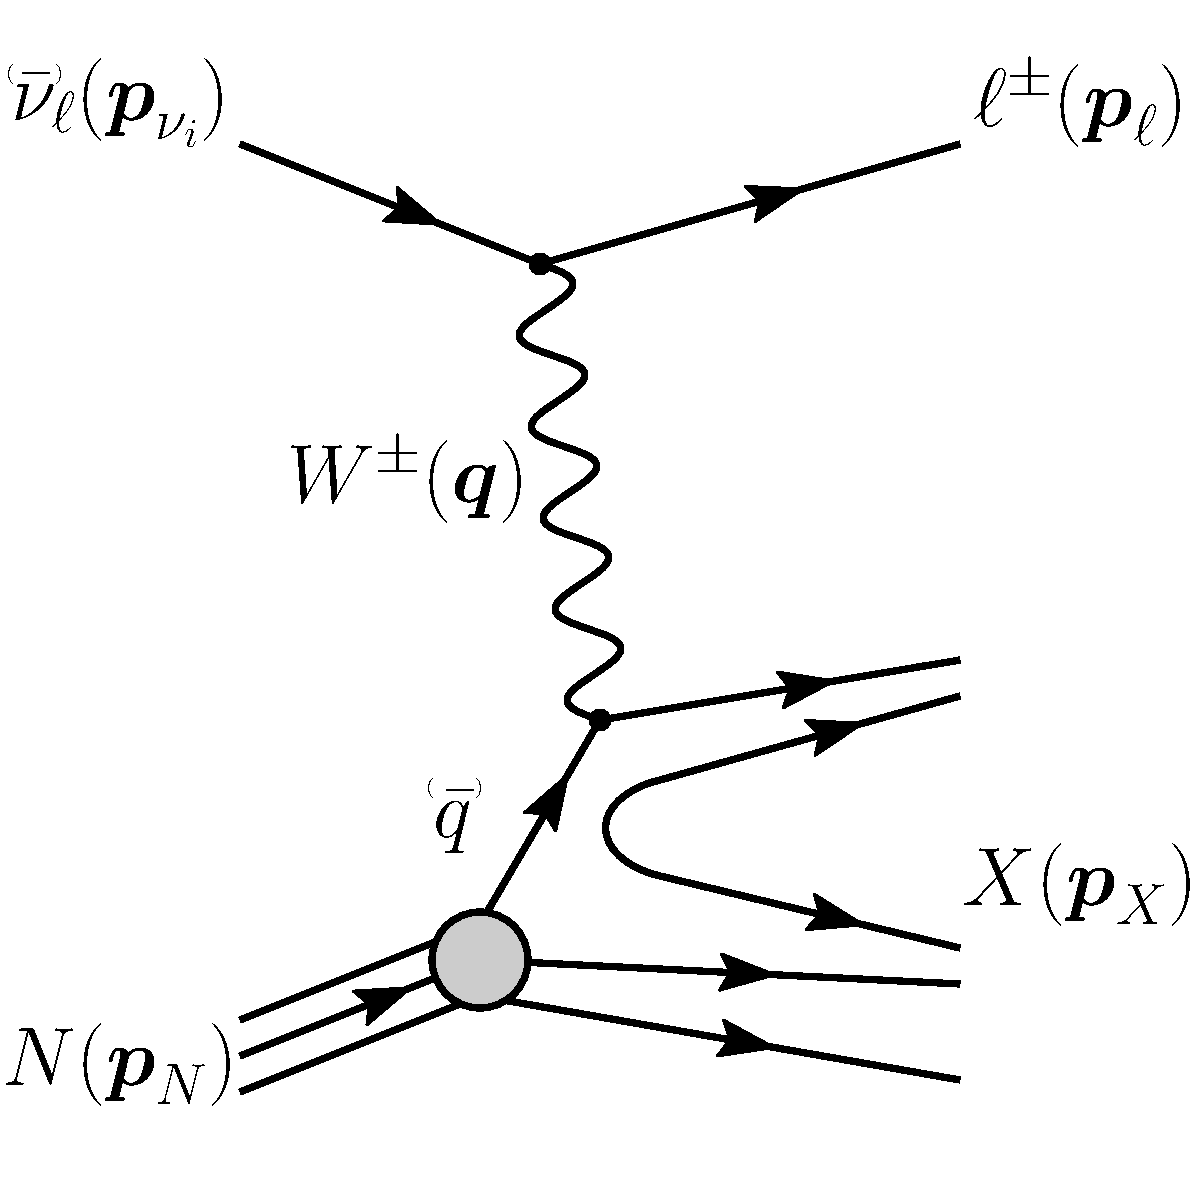
\includegraphics[width=0.4\linewidth]{figures/neutrinos_properties/feynman_DIS_CC_nu_new.pdf}
    \hspace{0.8cm}
    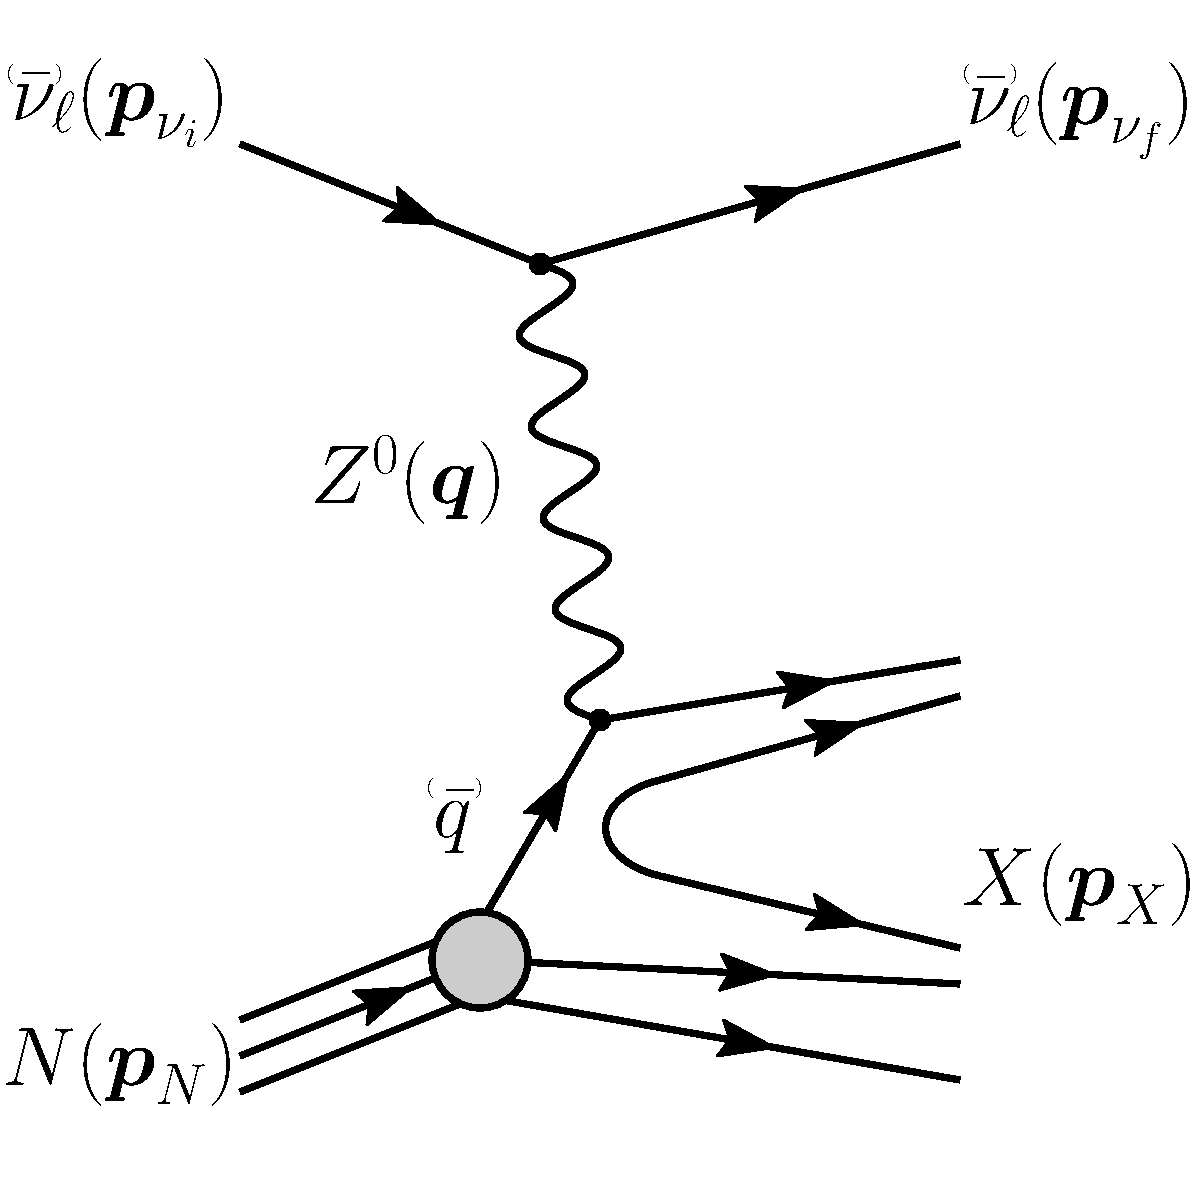
\includegraphics[width=0.4\linewidth]{figures/neutrinos_properties/feynman_DIS_NC_nu_new.pdf}
    \caption[Neutrino-nucleon deep inelastic scattering]{Feynman diagrams for deep inelastic scattering of a neutrino with a nucleon via charged-current (left) and neutral current (right) interactions. $\boldsymbol{p}_{\nu_i}$, $\boldsymbol{p}_{N}$ and $\boldsymbol{p}_{\nu_f}$, $\boldsymbol{p}_{l}$, $\boldsymbol{p}_{N}$ are the input and output four-momenta, while $\boldsymbol{q}$ is the momentum transfer. Taken from \cite{ATerliuk}.}
    \labfig{dis_feynman}
\end{figure}

At energies below \SI{5}{\gev}, \textbf{\textit{quasi-elastic scattering (QE)}} and \textbf{\textit{resonant scattering (RES)}} become important. At these energies the neutrinos interact with the approximately point-like nucleons, without breaking them up in the process. RES describes the process of a neutrino scattering off a nucleon producing an excited state of the nucleon in addition to a charged lepton. It is the dominant process from \SIrange{1.5}{5}{\gev} for neutrinos and from \SIrange{1.5}{8}{\gev} for antineutrinos. Below \SI{1.5}{\gev} QE is the dominant process, where protons are converted to neutrons in antineutrino interactions and vice-versa for neutrino interactions. Additionally, a charged lepton corresponding to the neutrino/antineutrino flavor is produced. The cross-sections of QE and RES scattering processes are not linear in energy and the transition region from QE/RES to DIS is poorly understood. The total cross-sections and their composition is shown in \reffig{neutrino_cross_sections}. It can be seen that the interaction cross-sections are very small at the order of $10^{-38}\mathrm{\,cm}^2$. This is the reason why very large volume detectors are required to measure atmospheric neutrinos with sufficient statistics to perform precision measurements of their properties.

\begin{figure*}[h]
	\centering
    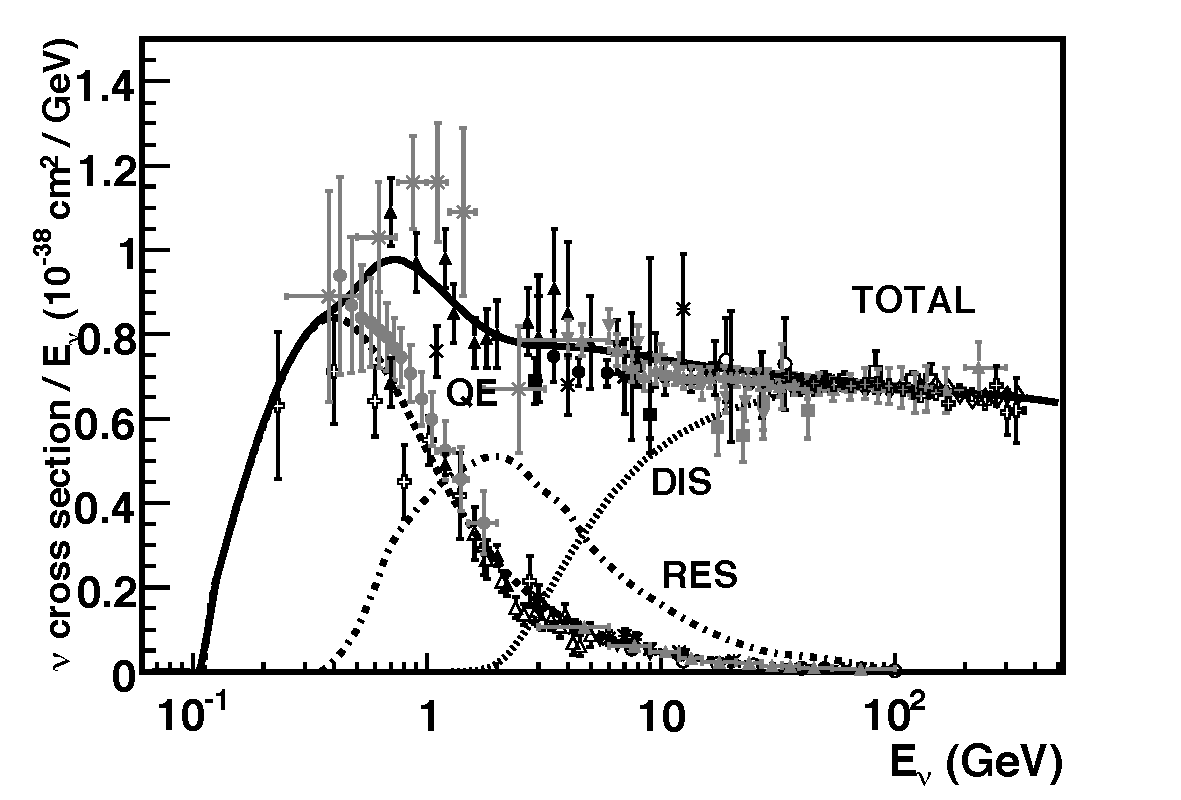
\includegraphics[width=0.495\linewidth]{figures/neutrinos_properties/cc_inclusive_nu.pdf}
    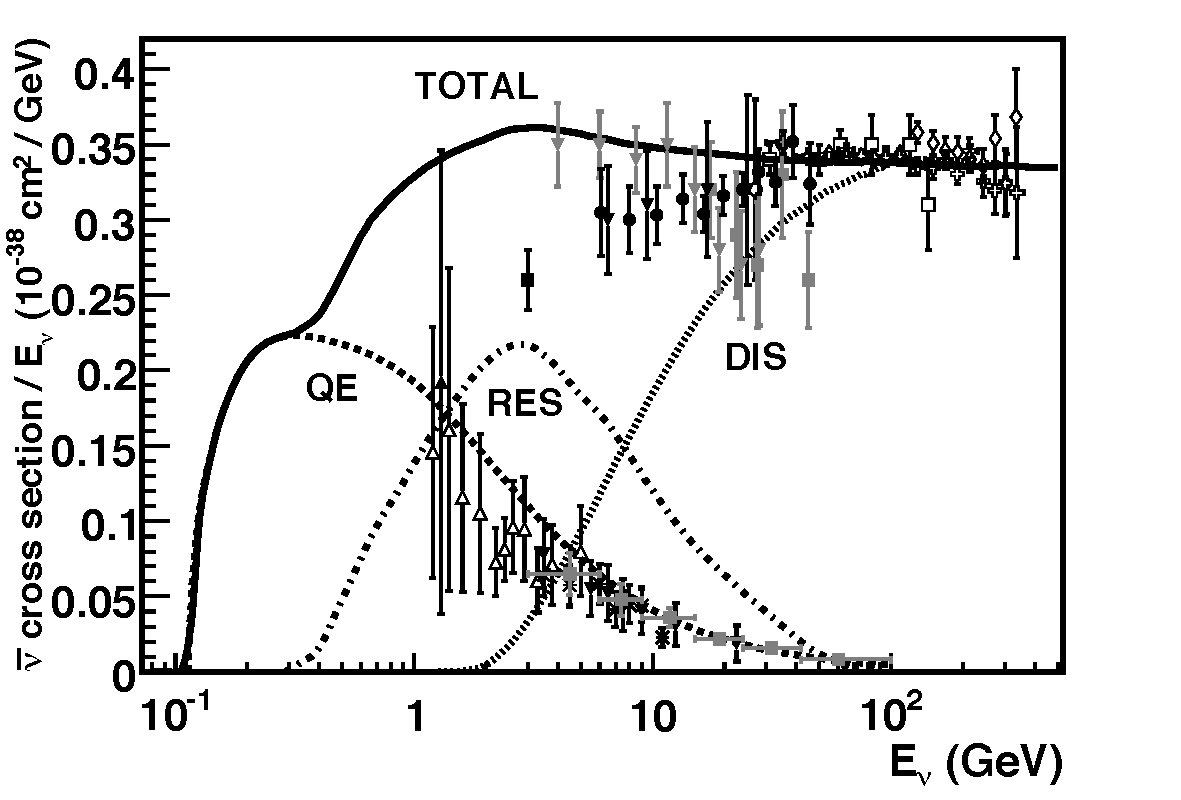
\includegraphics[width=0.495\linewidth]{figures/neutrinos_properties/cc_inclusive_nubar.pdf}
	\caption[Total inclusive neutrino-nucleon cross-sections]{Total neutrino (left) and antineutrino (right) per nucleon cross-section divided by neutrino energy plotted against energy.
    The three main scattering processes quasi-elastic scattering (QE), resonant scattering (RES), and deep-inelastic scattering (DIS) are shown. Taken from \cite{Formaggio_Cross_Sections}.}
    \labfig{neutrino_cross_sections}
\end{figure*}


\subsection{Heavy Neutral Lepton Production and Decay} \labsec{double_cascade_morphology}


For the search conducted in this work, both production and decay of the HNL are assumed to happen inside the detector, therefore probing decay lengths ranges at the scale of the detector size, which is below \SI{1000}{\meter}. Since the mixing with the first two generations of leptons is already strongly constrained as was discussed in \refsec{hnl_theory}, only the mixing with the tau neutrino will be considered in the following. Due to the effect of oscillations, described in \refsec{neutrino_oscillations}, the initial atmospheric muon neutrino flux provides a sizable tau neutrino flux at the detector.

\begin{figure}[h]
    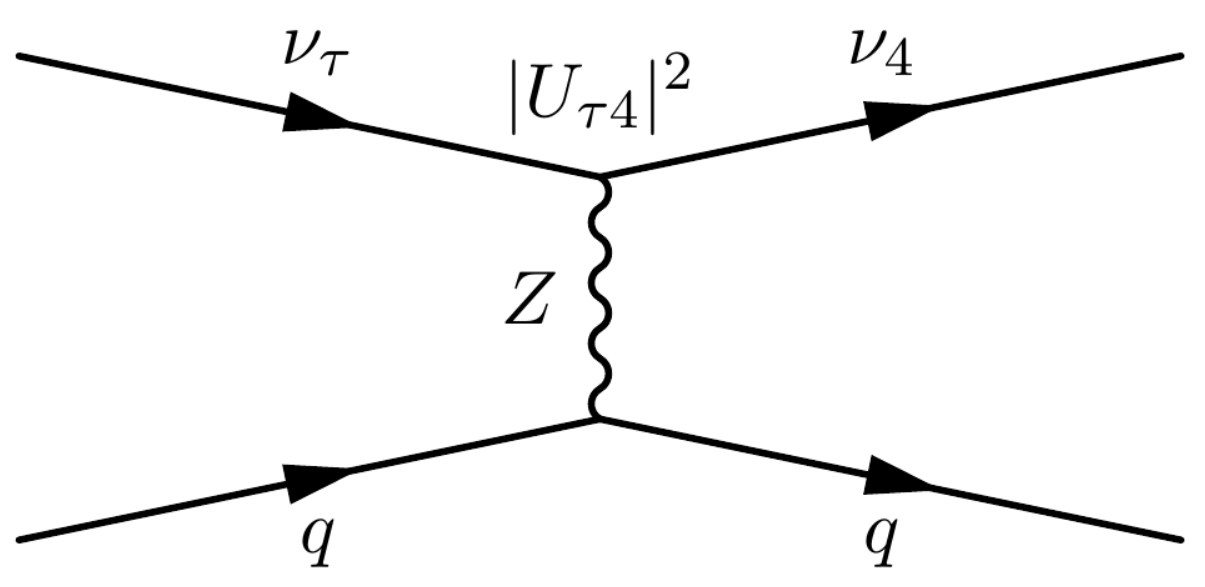
\includegraphics[width=0.5\textwidth]{figures/hnl_simulation/theory/feyn_diags_production.png}
    \caption[Feynman diagram of heavy neutral lepton production]{Feynman diagram of the HNL production. The heavy mass state is produced in the up-scattering of a tau neutrino.}
    \labfig{HNL_production}
\end{figure}

For a non-zero \ut4, the HNL can be produced through \textbf{up-scattering in the ice}. An incoming tau neutrinos scatters on an ice nucleus and transfers some of its kinetic energy to the heavy neutrino. The Feynman diagram of this process is shown in \reffig{HNL_production}. The custom NC cross-sections calculated for this purpose are explained in more detail in \refsec{custom_leptoninjector}, but are similar to the SM tau neutrino NC cross-sections, with a reduction scaling with the mixing \ut4 and energy dependent reductions, due to kinematic constraints because of the heavy neutrino mass. The scattering process produces a hadronic cascade, which will produce light in the detector.

\begin{figure}[h]
    \includegraphics{figures/hnl_simulation/theory/feyn_diags_decay.png}
    \caption[Feynman diagram of heavy neutral lepton decay]{Feynman diagram of the HNL decay. The heavy mass state can decay through neutral current interaction (left) into a tau neutrino and a charged lepton or quark pair, or through charged current interaction (right) into a tau lepton and a charged lepton or quark.}
    \labfig{HNL_decay}
\end{figure}

After a certain distance, the HNL will \textbf{decay in the ice}, where the possible decay channels considered in this work and the underlying, explicit calculations are discussed in \refsec{custom_leptoninjector}. The decay can be a CC or NC and both purely leptonic and leptonic+mesonic modes are possible. The Feynman diagrams of the decays can be seen in \refsec{HNL_decay}. Only the mass range relevant for this work is presented and mixing with $\nu_{e/\mu}$ is assumed to be negligible. Depending on the decay channel, an electromagnetic or a hadronic cascade is produced, while some energy is carried away by the invisible neutrino. The decay length of the HNL is defined by its proper lifetime\sidenote{A particle decay time follows an exponential distribution, with mean lifetime given by the proper lifetime. The proper lifetime is the lifetime in the rest frame of the particle.}, which is given by
\begin{equation}
    \tau_\mathrm{proper} = \frac{\hbar}{\Gamma_\mathrm{total}(m_4) \cdot |U_{\tau4}|^2}
    \;,
    \labeq{proper_lifetime_v0}
\end{equation}
where $\hbar$ is the reduced Planck constant, $\Gamma_\mathrm{total}(m_4)$ is the total decay width of the HNL for the given mass, and $|U_{\tau4}|^2$ is the mixing with the tau neutrino. The total decay width is the sum of the partial decay widths for all possible decay channels. The mean lab frame decay length is then given by
\begin{equation}
    L_\mathrm{decay} = \gamma v \tau_\mathrm{proper}
    \;,
    \labeq{decay_length}
\end{equation}
where $\gamma$ is the Lorentz factor of the HNL, defined by the kinetic energy. This will be further discussed on \refsec{custom_leptoninjector}. \reffig{hnl_decay_lengths} shows the mean decay lengths for an example mass of $m_4=\SI{0.6}{\gev}$ and several mixing values.

\begin{figure}[h]
    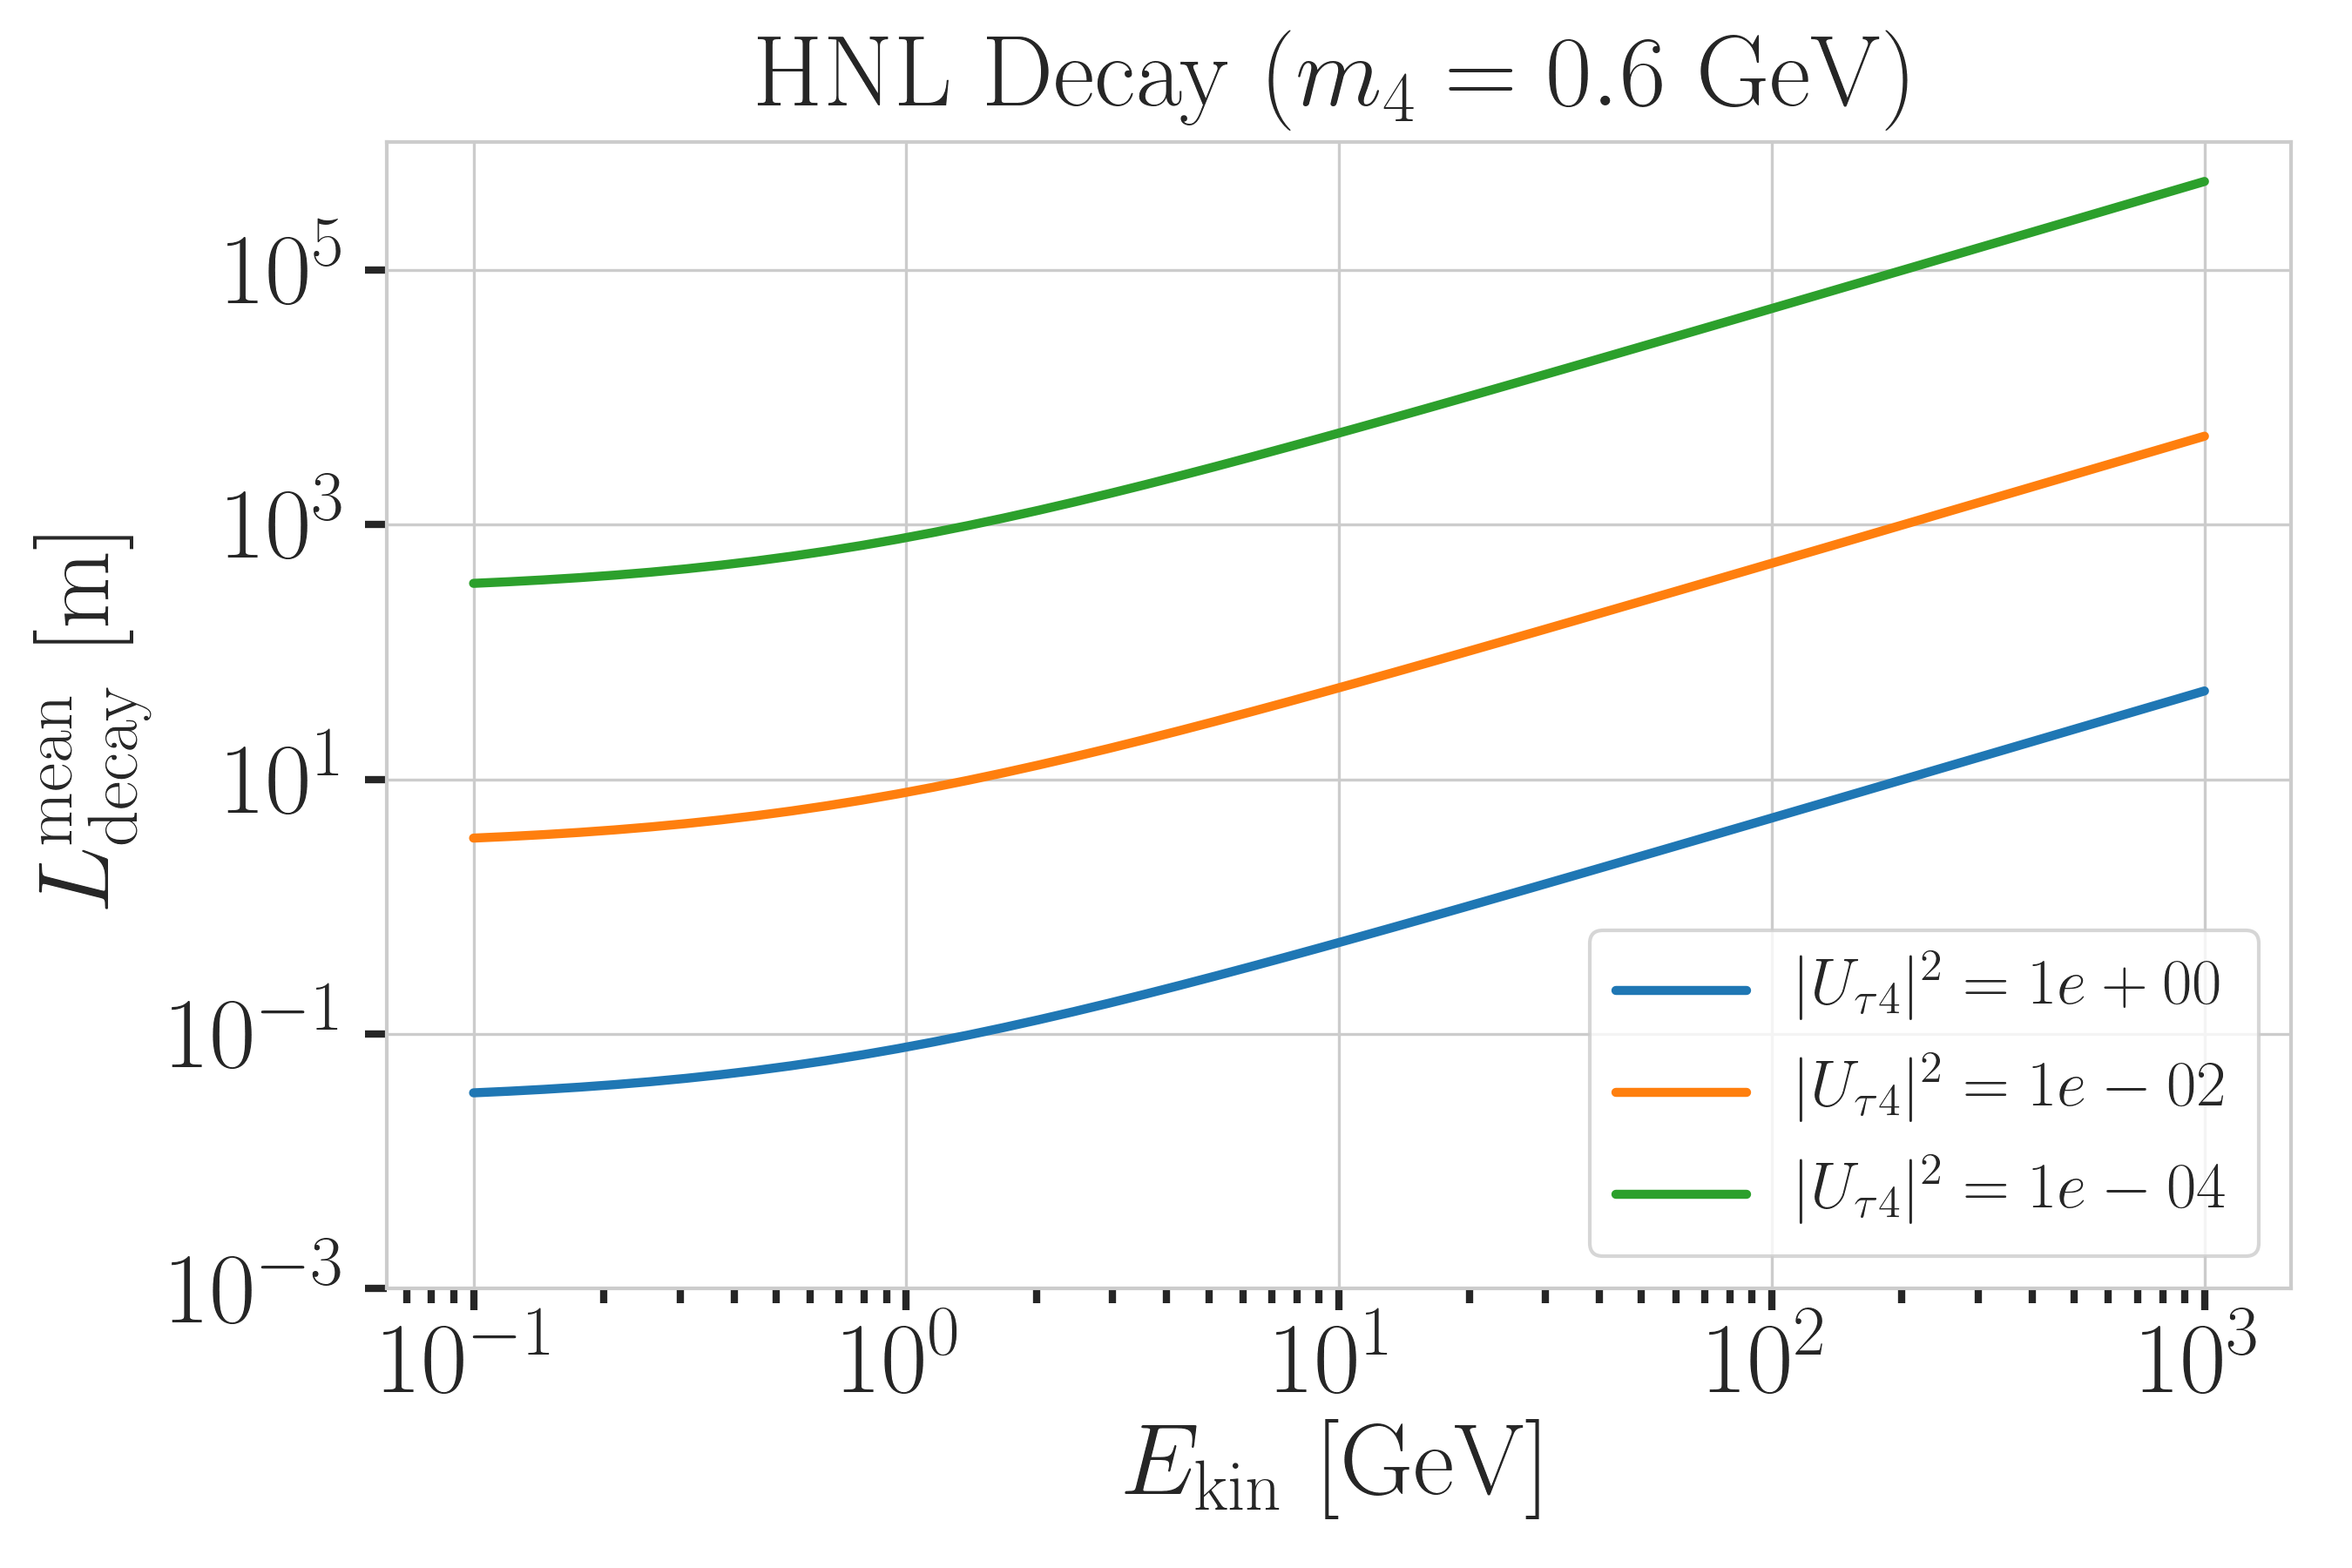
\includegraphics{figures/hnl_simulation/theory/decay_length_vs_energy_m4_6e-01.png}
    \caption[Theoretical mean HNL decay length (\SI{0.6}{\gev} mass)]{Theoretical mean decay length of the HNL for a mass of \SI{0.6}{\gev} and different mixing values.}
    \labfig{hnl_decay_lengths}
\end{figure}
